%% TO BE IMPLEMENTED:
  %      .def("alterSpokenMessage", &Character::alterSpokenMessage)
  %      .def("actionRunning", &Character::actionRunning)%

%        .def("abortAction", &Character::abortAction)
%        .def("successAction", &Character::successAction)
%        .def("disturbAction", &Character::actionDisturbed)
%        .def("setClippingActive", &Character::setClippingActive)
%        .def("getClippingActive", &Character::getClippingActive)
%        .def("callAttackScript", &Character::callAttackScript)
%        .def("callDefendScript", &Character::callDefendScript)

%% run makeindex luadocu.idx
\documentclass[a4paper,10pt,makeidx]{scrreprt}
\usepackage[ansinew]{inputenc}
\usepackage{amsmath}
\usepackage{graphicx}
\usepackage{makeidx}
\usepackage[dvips]{color}
\usepackage{boxedminipage}
\usepackage{listings}
\usepackage{hyperref}
\usepackage{multicol}
\usepackage{longtable}
\usepackage{pstricks}

\textwidth16cm \oddsidemargin0cm \evensidemargin0cm \topmargin-1cm
\textheight21cm
\newcommand{\com}[2]{\index{#1}\texttt{#1(}#2\texttt{)}}
\newcommand{\comm}[1]{\index{#1}\texttt{#1}}
\newcommand{\var}[1]{$\left\langle \text{\emph{#1}} \right\rangle$}
\newcommand{\lua}[1]{\index{#1}\texttt{\emph{#1}}}
\newcommand{\void}{\textsl{void }}
\newcommand{\lualist}[1]{\textsl{list (}#1\textsl{) }}
\newcommand{\integer}{\textsl{int }}
\newcommand{\double}{\textsl{double }}
\newcommand{\txt}{\textsl{text }}
\newcommand{\scripti}{\textsl{scrItem }}
\newcommand{\commoni}{\textsl{comItem }}
\newcommand{\bool}{\textsl{boolean }}
\newcommand{\effect}{\textsl{effStruct }}
\newcommand{\position}{\textsl{posStruct }}
\newcommand{\character}{\textsl{Character }}
\newcommand{\player}{\textsl{Player }}
\newcommand{\container}{\textsl{conStruct }}
\newcommand{\dialog}{\textsl{Dialog }}
\newcommand{\function}{\textsl{function }}
\newcommand{\weapon}{\textsl{wpnStruct }}
\newcommand{\armor}{\textsl{armStruct }}
\newcommand{\naturalarmor}{\textsl{natarmStruct }}
\newcommand{\tile}{\textsl{tleStruct }}
\newcommand{\datatable}{\textsl{dataTable }}
\newcommand{\ItemLookAt}{\textsl{ItemLookAt }}
\newcommand{\Skill}{\textsl{Skill }}
\makeindex
\begin{document}
\lstset{basicstyle=\small, keywordstyle=\ttfamily, identifierstyle=\ttfamily}
\title{Lua documentation for Illarion scripting\\v5.15}
\author{Martin \thanks{ \texttt{martin@illarion.org, http://www.illarion.org}},
pharse \thanks{ \texttt{pharse@illarion.org, http://www.illarion.org}},
vilarion \thanks{ \texttt{vilarion@illarion.org, http://www.illarion.org}}}
\date{2004-2006/2010-2014}
\maketitle
\tableofcontents
\chapter{General}
\section{Formalism}
System variables and variables of structures are accessed by ".".\\
Functions are called by ":".\\
If a function has no parameters, one still has to write ().\\
Lines that start with "?" refer to unclear commands.\\
Lines that start with "!" refer to suggested commands.\\
For variables, "\lua{r}:" in front of them means reading access, "\lua{rw}:" means reading and writing access.\\
Names in \comm{this font} refer to illarion-specific key words.\\
Names in \lua{this font} refer to lua-specific key words.\\
Names in \var{in this format} are placeholder and can be seen as variables.\\
Names in normal fixed font refer to a special choice of variables.\\
Names of functions are designed to be self explaining, therefore there are a lot of undocumented functions around.\\

Examples:\\
\begin{verbatim}
 XKoordinate=TargetItem.pos.x;
 User:talk(Character.say, "Hallo Welt!");
\end{verbatim}
\emph{Important note}: Lua is case sensitive.

\section{General introduction}
Everytime certain events happen (someone shift-clicks an object, a monster dies, someone looks at an
object, ... see the section about "entry points"), a script is started. The name of that script
is usually defined in the SQL-database in a separate row. For example, the table common, which
holds information about all items in illarion (weight, ...), has a row called com\_script,
which holds the name of the script that is linked to each item.
If someone shift-clicks an item, the lua-script that is linked to this item in common is
executed. This script then consists of several functions, defining what happens in certain cases: the item
can be used with another item (shift-clicks), with a character and so on. This means, a general item has the following
lua-file

\begin{verbatim}
       -- item.lua
 function UseItem(User, SourceItem)
     ...
 end

 function UseItemWithCharacter(User, SourceItem, Character)
     ...
 end

 function LookAtItem(User, Item)
     ...
 end
 ...
\end{verbatim}

Such a lua-file does not need all possible functions; if an item has no \com{LookAtItem}-function (LookAt=left-click),
it simply does nothing (special) when looked at. There are also entry points for magic and NPCs, which can
be found in the entry points section again.

\section{Variable types}
\begin{itemize}
        \item       \var{User}, \var{Originator}, \var{Character}: Character-type variables, see chapter "Characters".
        \item       \var{SourceItem}, \var{TargetItem}: Item-type variables, see chapter "Items".
        \item       \var{Pos}, \var{ItemPos}, \var{TargetItemPos}, \var{TargetPos}: Position-type variables, see chapter "Positions"
        \item       \datatable: Type that represents a Lua table, mapping data keys (strings) to data values (strings or integers).
        \item       \Skill: Type that represents a skill, embedded in Character like this: Character.\var{name}. Valid values for \var{name} are defined in the database in skills.skl\_name.
\end{itemize}

\chapter{Quickstart: Tutorials}
To provide you with a way to start very quickly with scripting simple things, here's a tutorial section.

\section{Level 0: Before we start}
Before you start, you need
\begin{itemize}
    \item Access to the script-SVN-repository; that includes free the tortoise SVN client or similar.
    \item A text editor (for starters, the Windows-Editor or Wordpad will do).
    \item Access to Illarion's testserver and the testclient and a character on the testserver with GM-rights.
    \item Creativity!
    \item Optional: DB access.
\end{itemize}

\section{Level 1: Your first script}
As your first script, we recommend to use the item with the ID 2. It is bound to the script named "{\tt I\_2\_mehl.lua}". Open it in your text editor and delete the whole file except for the following lines:
\begin{verbatim}
    function UseItem(User, SourceItem, ltstate)

    end
\end{verbatim}
What does this mean?

Every time someone "uses" (=shift clicks) an item with ID 2 (flour), the function {\tt UseItem(...)} inside the script {\tt I\_2\_mehl.lua} is called. The server provides this script with the following information:
\begin{itemize}
    \item {\tt User} contains all information about the character "using" the flour, like his position on the map, his hitpoints, skills, attributes and so on.
    \item {\tt SourceItem} contains all information about the "used" item---the flour in our case---like where it is on the map, what {\tt data}-value it has and so on.
    \item {\tt TargetItem} is only used in case you "used" the flour with some other item. In that case, it contains all information about the second item.
    \item {\tt ltstate} can be ignored for now as it is not important for our scripts.
\end{itemize}
Let's try the following script:
\begin{verbatim}
    function UseItem(User, SourceItem, ltstate)
        User:inform(User.name.." has used me!");
    end
\end{verbatim}
Commit this script to the svn-repository, log into the testserver (if you haven't already), reload the item-scripts by saying "{\tt !rd}" with your character and wait until it finishes with "***Definitions reloaded***". Then produce flour (by saying "{\tt !create 2}", you get one) and shift-click it. In my case, what appears is: {\tt Ciryon: Ciryon has used me!}

\chapter{Positions}

\section{Functions}
\position \var{position}=\com{position}{\integer \var{x},\integer \var{y},\integer \var{z}}
\begin{quote}
Creates position-structure for the point (x,y,z).\\
\end{quote}
\bool \position \var{posA} == \position \var{posB}
\begin{quote}
Compares two position structs. Returns \var{true} if they are equal, \var{false} otherwise.
\end{quote}
\txt \com{tostring}{\position \var{pos}}
\begin{quote}
Returns "(" .. pos.x .. ", " .. pos.y .. ", " .. pos.z .. ")".
\end{quote}

\section{Variables}
\lua{rw}: \integer \var{position}.\comm{x}\\
\lua{rw}: \integer \var{position}.\comm{y}\\
\lua{rw}: \integer \var{position}.\comm{z}\\
%\begin{quote}
\emph{Usage:} XCoordinate=User.pos.x
%\end{quote}

\section{Additional information}
Note that a position from a character struct is only a pointer. Thus it will change if the character changes its position. Example: \\
\begin{verbatim}
User:forceWarp( position(0,0,0) );
testPos = User.pos;							-- testPos is (0,0,0)
User:forceWarp( position(1,1,1) );		-- now User.pos AND testPos is (1,1,1)
\end{verbatim}

Avoid this by copying the single x,y and z coordinates in a new position struct.


\chapter{Characters}

\section{Functions}
\subsection{Text/Speech}
\void \var{character}:\com{talk}{\integer \var{texttype},\txt \var{text}}
\begin{quote}
       \var{texttype} can be \comm{Character.say}, \comm{Character.whisper} or \comm{Character.yell}.\\
       Lets a character say/whisper/yell some \var{text}.\\
       Example: \comm{User}:\com{talk}{\comm{Character.say}, "Hello world!"}
\end{quote}
\void \var{character}:\com{talk}{\integer \var{texttype},\txt \var{germanText}, \txt \var{englishText}}
\begin{quote}
       Same as \com{talk}{...} except that players will only hear speech in their own language.
\end{quote}
\void \var{character}:\com{inform}{\txt \var{Text}, \integer \var{informtype} = \comm{Character.mediumPriority}}\\
\void \var{character}:\com{inform}{\txt \var{germanText}, \txt \var{englishText}, \integer \var{informtype} = \comm{Character.mediumPriority}}
\begin{quote}
       Informs a player with a short \var{Text} and has no effect when used with other character types. Except for debugging the second syntax should be used to add native language support. Different priorities can be selected. These determine how prominent the \var{Text} is shown on the screen. Valid priorities are: \comm{Character.lowPriority}, \comm{Character.mediumPriority} as default if this parameter is omitted and \comm{Character.highPriority}.\\
       Examples: \comm{User}:\com{inform}{"Du bist betrunken.", "You are drunk."}\\
       \phantom{Examples: }\comm{User}:\com{inform}{"A raindrop falls on your head.", \comm{Character.lowPriority}} \\
\end{quote}
\void \var{character}:\com{introduce}{\player \var{player}}
\begin{quote}
       Introduces \var{player} to \var{character} if character is a player as well. Otherwise it has no effect.
\end{quote}
\void \var{character}:\com{move}{\integer \var{direction},\bool \var{active move}}
\begin{quote}
       \var{character} makes a step into \var{direction}.
       \var{active move} is true if the move was done actively (normal case) and false otherwise.
        \begin{figure}[htp]
            \begin{center}
                \scalebox{1} % Change this value to rescale the drawing.
                {
                \begin{pspicture}(0,-1.52)(6.02,1.52)
                \definecolor{color128}{rgb}{0.6,0.6,0.6}
                \psline[linewidth=0.04cm](0.0,0.0)(3.0,1.5)
                \psline[linewidth=0.04cm](3.0,1.5)(6.0,0.0)
                \psline[linewidth=0.04cm](0.0,0.0)(3.0,-1.5)
                \psline[linewidth=0.04cm](3.0,-1.5)(6.0,0.0)
                \psline[linewidth=0.04cm](1.0,0.5)(4.0,-1.0)
                \psline[linewidth=0.04cm](2.0,1.0)(5.0,-0.5)
                \psline[linewidth=0.04cm](2.0,-1.0)(5.0,0.5)
                \psline[linewidth=0.04cm](1.0,-0.5)(4.0,1.0)
                \usefont{T1}{ptm}{m}{n}
                \rput(2.0159376,0.51){N=0}
                \usefont{T1}{ptm}{m}{n}
                \rput(3.0103126,1.01){NE=1}
                \usefont{T1}{ptm}{m}{n}
                \rput(3.98875,0.51){E=2}
                \usefont{T1}{ptm}{m}{n}
                \rput(4.97375,0.01){SE=3}
                \usefont{T1}{ptm}{m}{n}
                \rput(3.9725,-0.49){S=4}
                \usefont{T1}{ptm}{m}{n}
                \rput(2.936875,-0.99){SW=5}
                \usefont{T1}{ptm}{m}{n}
                \rput(1.9507812,-0.49){W=6}
                \usefont{T1}{ptm}{m}{n}
                \rput(0.984375,0.01){NW=7}
                \psline[linewidth=0.03cm,linecolor=color128,dotsize=0.07055555cm 2.0,arrowsize=0.05291667cm 2.0,arrowlength=1.4,arrowinset=0.4]{*->}(3.0,0.0)(2.2,0.4)
                \psline[linewidth=0.03cm,linecolor=color128,dotsize=0.07055555cm 2.0,arrowsize=0.05291667cm 2.0,arrowlength=1.4,arrowinset=0.4]{*->}(3.0,0.0)(3.8,-0.4)
                \psline[linewidth=0.03cm,linecolor=color128,dotsize=0.07055555cm 2.0,arrowsize=0.05291667cm 2.0,arrowlength=1.4,arrowinset=0.4]{*->}(3.0,0.0)(2.3,-0.4)
                \psline[linewidth=0.03cm,linecolor=color128,dotsize=0.07055555cm 2.0,arrowsize=0.05291667cm 2.0,arrowlength=1.4,arrowinset=0.4]{*->}(3.0,0.0)(3.7,0.4)
                \psline[linewidth=0.03cm,linecolor=color128,dotsize=0.07055555cm 2.0,arrowsize=0.05291667cm 2.0,arrowlength=1.4,arrowinset=0.4]{*->}(3.0,0.0)(3.0,0.8)
                \psline[linewidth=0.03cm,linecolor=color128,dotsize=0.07055555cm 2.0,arrowsize=0.05291667cm 2.0,arrowlength=1.4,arrowinset=0.4]{*->}(3.0,0.0)(3.0,-0.8)
                \psline[linewidth=0.03cm,linecolor=color128,dotsize=0.07055555cm 2.0,arrowsize=0.05291667cm 2.0,arrowlength=1.4,arrowinset=0.4]{*->}(3.0,0.0)(1.6,0.0)
                \psline[linewidth=0.03cm,linecolor=color128,dotsize=0.07055555cm 2.0,arrowsize=0.05291667cm 2.0,arrowlength=1.4,arrowinset=0.4]{*->}(3.0,0.0)(4.4,0.0)
                \end{pspicture}
                }
            \end{center}
        \caption{The 8 possible directions}\label{directions}
        \end{figure}
\end{quote}
\void \var{character}:\com{turn}{\integer \var{direction}}\\
\void \var{character}:\com{turn}{\position \var{position}}
\begin{quote}
    Turns \var{character} into the given \var{direction} or towards the given \var{position}.
\end{quote}
\txt \var{character}:\com{alterMessage}{\txt \var{Text},\integer \var{LanguageSkill}}
\begin{quote}
       Returns the altered \var{Text} with respect to the \var{LanguageSkill} given.
\end{quote}
\void \var{character}:\com{sendCharDescription}{\integer \var{id}, \txt \var{text}}
\begin{quote}
Shows the \var{text} as character description of the character with ID \var{id} (just next to the avatar) only to this \var{character}.
\end{quote}
\void \var{character}:\com{sendBook}{\integer \var{id}}
\begin{quote}
Tells the client to display book \var{id} for \var{character}. Books are stored as client resources.
\end{quote}

\subsection{Skills and Attributes}
\emph{NOTE:} There are two kinds of attributes: fixed and variable ones. All attributes that are not meant to develop during the game are fixed, e.g. strength, perception, age, sex etc.

On the other hand there are the variable attributes, e.g. any skill (of course), hitpoints, mana etc. Any change to those will be permanently written to the database.

Any change to fixed attributes is only temporary and will be null upon the next login. Example: You want to create an amulet that gives a +2 STR bonus when worn. It does not suffice to change the strength when the amulet is put on, you have to use a Long Time Effect that does the change again after a login (and checks if the amulet is still in its place).
\\\\
\txt \var{character}:\com{getSkillName}{\Skill \var{skill}}
\begin{quote}
       Returns the name of the given \var{skill} in the player's language.
\end{quote}
\integer \var{character}:\com{getSkill}{\Skill \var{skill}}\\
\textsl{Character:skillvalue} \var{character}:\com{getSkillValue}{\Skill \var{skill}}
\begin{quote}
       skillvalue is a table with two fields, major and minor, representing the skill and the minor skill.
\end{quote}
\integer \var{character}:\com{setSkill}{\Skill \var{skill}, \integer \var{major}, \integer \var{minor}}
\begin{quote}
       Directly sets major and minor skill. Returns the new major skill. If the skill does not exist in the database, nothing is set and 0 is returned.
\end{quote}
\integer \var{character}:\com{increaseSkill}{\Skill \var{skill}, \integer \var{value}}\\
\integer \var{character}:\com{increaseMinorSkill}{\Skill \var{skill}, \integer \var{value}}
\begin{quote}
       Increase major and minor skill, respectively. Return the new major skill. If the skill does not exist in the database, nothing is increased and 0 is returned.
\end{quote}
\void \var{character}:\com{learn}{\Skill \var{skill}, \integer \var{actionPoints},\integer \var{learnLimit}}
\begin{quote}
       \var{skill}: Constant of the skill.\\
       \var{actionPoints}: Number of actionPoints used up for the action which resulted in learning.\\
       \var{learnLimit}: The skill will not be advanced beyond this limit and never beyond 100.\\
\end{quote}
\integer \var{character}:\com{increaseAttrib}{\txt \var{AttribName}, \integer \var{value}}
\begin{quote}
       Increases the attribute given (see below) and returns the new attribute value. Use \var{value}=0 to read the attribute's value. Note
       that this command also sends a player update to all characters in range if necessary.
\end{quote}
\void \var{character}:\com{setAttrib}{\txt \var{AttribName}, \integer \var{value}}
\begin{quote}
       \var{AttribName} can be:
       "sex", "age", "body\_height", "attitude", "luck", "strength", "dexterity",
       "constitution", "agility", "intelligence", "perception", "willpower", "essence", "foodlevel", "hitpoints",
       "mana", "poisonvalue".
       And "sex" can be:
       Character.male, Character.female

       Be aware that any attribute change to fixed attributes like "strength" will only last for the current session and will be reset to the database value upon the next login.
\end{quote}
\bool \var{character}:\com{isBaseAttributeValid}{\txt \var{attribute}, \integer \var{value}}
\begin{quote}
Returns whether \var{value} is acceptable for the given \var{attribute} and the race of the character, respecting limits given in table raceattr.
\end{quote}
\integer \var{character}:\com{getBaseAttributeSum}{}
\begin{quote}
Returns the current sum of the eight primary attributes: agility, constitution, dexterity, essence, intelligence, perception, strength and willpower.
\end{quote}
\integer \var{character}:\com{getMaxAttributePoints}{}
\begin{quote}
Returns the value which \com{getBaseAttributeSum}{} needs to result in, so that the base attributes can be saved. Can be used to make tests before actually trying to save the base attributes.
\end{quote}
\integer \var{character}:\com{getBaseAttribute}{\txt \var{attribute}}
\begin{quote}
Returns the base value of the given \var{attribute}, that is the value that this attribute normally has, when no special effects are active.
\end{quote}
\bool \var{character}:\com{setBaseAttribute}{\txt \var{attribute}, \integer \var{value}}
\begin{quote}
Sets the base value of the given \var{attribute} and returns \var{true} if 
\com{isBaseAttributeValid}{...} would return \var{true}. Otherwise is a no-op and returns \var{false}.
\end{quote}
\bool \var{character}:\com{increaseBaseAttribute}{\txt \var{attribute}, \integer \var{amount}}
\begin{quote}
If \com{isBaseAttributeValid}{...} would return \var{true}, increases or decreases the base value of the given \var{attribute} and returns \var{true}. Otherwise is a no-op and returns \var{false}.
\end{quote}
\bool \var{character}:\com{saveBaseAttributes}{}
\begin{quote}
Saves the eight primary base attributes to the database, iff \com{getBaseAttributeSum}{} == \com{getMaxAttributePoints}{}. On failure resets primary attribute values to database values. Returns whether the operation was successful or not.
\end{quote}
\void \var{character}:\com{setSkinColor}{\integer \var{red}, \integer \var{green}, \integer \var{blue}}
\begin{quote}
    Sets the color of the skin to the given rgb-values. \var{red}, \var{green} and \var{blue} must be between 0 and 255.
\end{quote}
\void \var{character}:\com{setHairColor}{\integer \var{red}, \integer \var{green}, \integer \var{blue}}
\begin{quote}
    Sets the color of the hair and beard to the given rgb-values. \var{red}, \var{green} and \var{blue} must be between 0 and 255.
\end{quote}
\integer, \integer, \integer \var{character}:\com{getSkinColor}{}
\begin{quote}
    Returns the \var{red}, \var{green} and \var{blue} values of the skin color, each being between 0 and 255.
\end{quote}
\integer, \integer, \integer \var{character}:\com{getHairColor}{}
\begin{quote}
    Returns the \var{red}, \var{green} and \var{blue} values of the hair color, each being between 0 and 255.
\end{quote}
\void \var{character}:\com{setHair}{\integer \var{hairID}}
\begin{quote}
    Returns the ID of the present hair, 0 for no hair.
\end{quote}
\void \var{character}:\com{setBeard}{\integer \var{beardID}}
\begin{quote}
    Returns the ID of the present beard, 0 for no beard.
\end{quote}
\integer \var{character}:\com{getHair}{}
\begin{quote}
    Returns the ID of the present hair, 0 for no hair.
\end{quote}
\integer \var{character}:\com{getBeard}{}
\begin{quote}
    Returns the ID of the present beard, 0 for no beard.
\end{quote}
\integer \var{character}:\com{setRace}{\integer \var{race}}
\begin{quote}
    Temporarily sets the race of a character. See table \ref{raceIDs} for details. 
\end{quote}
\integer \var{character}:\com{getRace}{}
\begin{quote}
       Returns the race of a character. See table \ref{raceIDs} for details.
       \begin{table}
\begin{tabular}{lc|lc|lc}
    Name & \var{rID} & Name & \var{rID} & Name & \var{rID}  \\ \hline
    human & 0 & blackwolf & 41 & blacktroll & 80\\
    dwarf & 1 & greywolf & 42 & redtroll & 81\\
    halfling & 2 & redwolf & 43 & blackzombie & 82\\
    elf & 3 & redraptor & 48 & transparentzombie & 83\\
    orc & 4 & silverbear & 49 & redzombie & 84\\
    lizardman & 5 & blackbear & 50 & blackhellhound & 85\\
    gnome & 6 & bear & 51 & transparenthellhound & 86\\
    troll & 9 & raptor & 52 & greenhellhound & 87\\
    mumie & 10 & zombie & 53 & redhellhound & 88\\
    skeleton & 11 & hellhound & 54 & redimp & 89\\
    beholder & 12 & imp & 55 & blackimp & 90\\
    blackbeholder & 13 & irongolem & 56 & blueirongolem & 91\\
    transparentbeholder & 14 & ratman & 57 & redratman & 92\\
    brownmummy & 15 & dog & 58 & greenratman & 93\\
    bluemummy & 17 & beetle & 59 & blueratman & 94\\
    sheep & 18 & fox & 60 & reddog & 95\\
    spider & 19 & slime & 61 & greydog & 96\\
    demonskeleton & 20 & chicken & 62 & blackdog & 97\\
    redspider & 21 & bonedragon & 63 & greenbeetle & 98\\
    greenspider & 22 & blackbonedragon & 64 & copperbeetle & 99\\
    bluespider & 23 & redbonedragon & 65 & redbeetle & 100\\
    pig & 24 & transparentbonedragon & 66 & goldbeetle & 101\\
    boar & 25 & greenbonedragon & 67 & greyfox & 102\\
    transparentspider & 26 & bluebonedragon & 68 & redslime & 103\\
    wasp & 27 & goldbonedragon & 69 & blackslime & 104\\
    redwasp & 28 & redmummy & 70 & transparentslime & 105\\
    stonegolem & 30 & greymummy & 71 & brownchicken & 106\\
    brownstonegolem & 31 & blackmummy & 72 & redchicken & 107\\
    redstonegolem & 32 & goldmummy & 73 & blackchicken & 108\\
    silverstonegolem & 33 & transparentskeleton & 74 &  & \\
    transparentstonegolem & 34 & blueskeleton & 75 &  & \\
    cow & 37 & greenskeleton & 76 &  & \\
    bull & 38 & goldgolem & 77 &  & \\
    wolf & 39 & goldskeleton & 78 &  & \\
    transparentwolf & 40 & bluetroll & 79 &  & \\
\end{tabular}
\caption{List of available races with Race-IDs (\var{rID})}\label{raceIDs}
\end{table}
\end{quote}
\integer \var{character}:\com{getMonsterType}{}
\begin{quote}
       Returns the monster-ID of a monster. For a list of the current monster-IDs, please consult the database or one of the other developers.
\end{quote}

\integer \var{character}:\com{getFaceTo}{}
\begin{quote}
       Returns an integer between 0 and 7 inclusively that indicates the direction the character is facing to. For a list of the directions, see Fig.(\ref{directions}).
\end{quote}
\integer \var{character}:\com{getType}{}
\begin{quote}
       Returns Character.player for players, Character.monster for monsters and Character.npc for NPCs.
\end{quote}
\void \var{character}:\com{increasePoisonValue}{\var{value}}\\
\integer \var{character}:\com{getPoisonValue}{}\\
\void \var{character}:\com{setPoisonValue}{\integer \var{value}}\\
\integer \var{character}:\com{getMentalCapacity}{}\\
\void \var{character}:\com{setMentalCapacity}{\integer \var{value}}\\
\void \var{character}:\com{increaseMentalCapacity}{\integer \var{value}}\\
\integer \var{character}:\com{getMagicType}{}
\begin{quote}
       returns MagicType
\end{quote}
\void \var{character}:\com{setMagicType}{\integer \var{MagicType}}
\begin{quote}
       MagicType: "mage"=0, "priest"=1, "bard"=2, "druid"=3
\end{quote}
\integer \var{character}:\com{getMagicFlags}{\integer \var{MagicType}}\\
\void \var{character}:\com{teachMagic}{\integer \var{MagicType},\integer \var{MagicFlag}}\\
\integer \var{character}:\com{getPlayerLanguage}{}
\begin{quote}
       Returns the player's language: Player.german or Player.english.
\end{quote}

\subsection{Quest progress}
\void \var{character}:\com{setQuestProgress}{\integer  \var{questID},\integer  \var{progress}}
\begin{quote}
       A questprogress can be set for a specific quest.
\end{quote}
\integer\var{progress}[, \integer\var{time}] \var{character}:\com{getQuestProgress}{\integer \var{questID}}
\begin{quote}
       Returns the \var{progress} for a specific quest. Optionally also returns the \var{time} when this progress was last set as Unix timestamp.
\end{quote}
\subsection{Item handling}
\integer \var{character}:\com{createItem}{\integer \var{itemID},\integer \var{count},\integer \var{quality}, \datatable \var{data}}
\begin{quote}
       Item is created in the belt or backpack of \var{character}.
       If that is not possible, the items will not be created.
       The function returns an integer that gives the number of items that cannot be created.
       \comm{world}:\comm{createItemFromId} might be a good choice in addition.
\end{quote}
\void \var{character}:\com{createAtPos}{\integer \var{Position\_body},\integer \var{itemId},\integer \var{count}}
\begin{quote}
       Creates an item at a special body position (see below).
\end{quote}
\void \var{character}:\com{changeQualityAt}{\integer \var{Position\_body},\integer \var{qly-amount}}
\begin{quote}
       Changes the quality by amount at position\_body.
\end{quote}
\integer \var{character}:\com{eraseItem}{\integer \var{itemID},\integer \var{count}}\\
\integer \var{character}:\com{eraseItem}{\integer \var{itemID},\integer \var{count}, \datatable \var{data}}
\begin{quote}
       \var{count} item with \var{itemID} (=number!) are erased from the \var{character} inventory.
       You have no influence on which items are deleted, you can just determine ID and number. The
       return value contains the amount of items that could not be deleted. In case the optional
       \var{data} parameter is set, only items that include these data values are deleted.
       If the data table is empty however, only items without data are erased.
\end{quote}
\integer \var{character}:\com{countItem}{\integer \var{itemID}}\\
\integer \var{character}:\com{countItemAt}{\txt \var{location},\integer \var{itemID}}\\
\integer \var{character}:\com{countItemAt}{\txt \var{location},\integer \var{itemID},\datatable \var{data}}
\begin{quote}
       Counts only at a certain position; \var{character}:countItemAt("all",...) is the same as \var{character}:\com{countItem}{...}\\
       \var{location} can be "all", "belt", "body", "backpack". The variant with \var{data} does only count items that include these data values.
       If the data table is empty however, only items without data are counted.
\end{quote}
\void \var{character}:\com{increaseAtPos}{\integer \var{Position\_body},\integer \var{count}}\\
\void \var{character}:\com{swapAtPos}{\integer \var{Position\_body},\integer \var{itemID},\integer \var{quality}}
\begin{quote}
       Position\_body: {\tt BACKPACK=0, HEAD=1, NECK=2, BREAST=3, HANDS=4,
       LEFT\_TOOL=5, RIGHT\_TOOL=6, FINGER\_LEFT\_HAND=7,
       FINGER\_RIGHT\_HAND=8, LEGS=9, FEET=10, COAT=11,
       LAST\_WEARABLE=11}\\
       To be combined with \var{Item}:\com{getType}{ }.\\
       See fig.(\ref{itemtypes}).\\
       If quality=0, then the quality remains the same.
\end{quote}
\scripti \var{character}:\com{getItemAt}{\integer \var{Position\_body}}
\begin{quote}
       \var{Position\_body}: {\tt
       Character.backpack=0, Character.head=1, Character.neck=2,\\
       Character.breast=3, Character.hands=4, Character.left\_tool=5,\\
       Character.right\_tool=6, Character.finger\_left\_hand=7, \\
       Character.finger\_right\_hand=8, Character.legs=9,\\
       Character.feet=10, Character.coat=11, Character.belt\_pos\_1=12,\\
       Character.belt\_pos\_2=13, Character.belt\_pos\_3=14, \\
       Character.belt\_pos\_4=15, Character.belt\_pos\_5=16,\\
       Character.belt\_pos\_6=17}\\
       This returns a ScriptItemStruct. See fig. (\ref{itemtypes}).
\end{quote}
\lualist{\scripti} \var{character}:\com{getItemList}{\integer \var{ItemID}}
\begin{quote}
Returns a list with all items of this \var{ItemID}.
\end{quote}
\container \var{character}:\com{getBackPack}{}
\begin{quote}
       Returns a container-item (which is different from scriptitem and commonitem). Containeritems can be used to pick out items which are placed in it. See \var{Container}:\com{takeItemNr}{\var{itempos},\var{count}}.
\end{quote}
\container \var{character}:\com{getDepot}{\integer \var{depotId}}
\begin{quote}
       Returns a container-item (the depot of that Character). Containeritems can be used to pick out items which are placed in it. See \var{Container}:\com{takeItemNr}{\var{itempos},\var{count}}.
\end{quote}

\subsection{All the rest}
\bool \var{character}:\com{isNewPlayer}{}
\begin{quote}
       Returns whether \var{character} is a new player or not. The exact behaviour is defined in the database function is\_new\_player.
\end{quote}
\bool \var{character}:\com{isInRange}{\character \var{character2},\integer \var{Distance}}
\begin{quote}
       Returns true if \var{character2} is within \var{Distance} of \var{character}, else false.
\end{quote}
\integer \var{character}:\com{distanceMetric}{\character \var{character2}}
\begin{quote}
       Returns distance.\\
       Very similar to isInRange, but much more flexible. Better use distanceMetric.
\end{quote}
\integer \var{character}:\com{distanceMetricToPosition}{\position \var{Position}}
\begin{quote}
       Returns the distance from \var{character} to \var{Position}.
\end{quote}
\bool \var{character}:\com{isInRangeToPosition}{\position \var{Position},\integer \var{distance}}
\begin{quote}
       Returns \lua{true} when the \var{character} is within the \var{distance} to \var{position} and \lua{false} otherwise.
\end{quote}
\void \var{character}:\com{warp}{\position \var{Position}}
\begin{quote}
       "Position" is a position-structure as described above.
\end{quote}
\void \var{character}:\com{forceWarp}{\position \var{Position}}
\begin{quote}
       "Position" is a position-structure as described above. This command works exactly as warp, but it ignores any non-passable flags on the target position. That means that you can warp onto e.g. water using this command.
\end{quote}
\void \var{character}:\com{startMusic}{\integer \var{Number}}
\begin{quote}
       Starts music \var{Number} for \var{character}, with 0 meaning silence.
       This overrides the default music given by the map until logout or a call of \var{character}:\com{defaultMusic}{}
\end{quote}
\void \var{character}:\com{defaultMusic}{}
\begin{quote}
       Plays the default music for \var{character} as defined by the map.
\end{quote}
\bool \var{character}:\com{isAdmin}{}
\begin{quote}
       Returns \lua{true} if that character is admin (GM) and \lua{false} otherwise.
\end{quote}
\void \var{character}:\com{setClippingActive}{\bool \var{status}}
\begin{quote}
       \var{status} must be either \lua{true} (walking through walls disabled) or \lua{false}; this enables the character to walk on
       fields where he usualy can't walk (water, walls, ...). Please use with care: This has to be turned OFF again!
\end{quote}
\bool \var{character}:\com{getClippingActive}{}
\begin{quote}
       Returns \lua{true} or \lua{false}.
\end{quote}
\integer \var{character}:\com{idleTime}{}
\begin{quote}
       If \var{character} is a player, returns the number of seconds they are idle. Returns 0 otherwise.
\end{quote}
\bool \com{isValidChar}{\character \var{char}}
\begin{quote}
       Returns \lua{true} iff \var{char} is still valid and safe to use. Validity has to be checked if \var{char} is used in another entrypoint call than the one where it was originally obtained, since a player might have logged out, an NPC might have been deleted and a monster might have been killed in the meantime.
\end{quote}
\bool \var{character}:\com{pageGM}{\txt \var{ticket}}
\begin{quote}
       Returns \lua{true} iff \var{ticket} is successfully logged as message to the GM team. Differing from the normal !gm command, the originating player is not informed about success.
\end{quote}
\void \var{character}:\com{logAdmin}{\txt \var{message}}
\begin{quote}
       Writes \var{message} for the given user into the server log using the admin facility. Only used to record GM actions.
\end{quote}

\section{Variables}
\lua{r}:  \txt \var{character}.\comm{lastSpokenText}
\begin{quote}
Returns this characters last spoken line of text
\end{quote}
\lua{r}: \position \var{character}.\comm{pos}
\begin{quote}
       Position-structure
\end{quote}
\lua{r}: \txt \var{character}.\comm{name}\\
\lua{r}: \integer \var{character}.\comm{id}\\
\lua{r}: \bool \var{character}.\comm{attackmode}
\begin{quote}
       \lua{true} if character currently attacks, \lua{false} otherwise.
\end{quote}
\lua{rw}: \integer \var{character}.\comm{activeLanguage}
\begin{quote}
       "common language"=0, "human language"=1, "dwarf language"=2,
       "elf language"=3, "lizard language"=4, "orc language"=5,
       "halfling language"=6, "fairy language"=7, "gnome language"=8,
       "goblin language"=9, "ancient language"=10
\end{quote}
\lua{rw}: \integer \var{character}.\comm{movepoints}
\begin{quote}
		A character has usually (when being idle) 21 movepoints.
		Every action like talking, fighting, using etc. needs at least ca. 6
		movepoints. The reduction of movepoints depends on the character's
		agility. The regeneration is for all the same: +10 per second.
		A greater amount than 21 movepoints is not possible as it is immediately
		set again to 21.
\end{quote}

\chapter{Containers}
Some items can contain other items. These are for example a character's backpack and depot. There are multiple functions to get access to such a container variable. Here is what you can do with those:

\section{Functions}

\bool, \scripti, \container \var{Container}:\com{viewItemNr}{\integer \var{itempos}}
\begin{quote}
       Returns three values in that specific order: \comm{bool} \var{success}, \comm{structitem} \var{item}, \comm{containeritem} \var{container}.
       \var{success} is \lua{true} if Lua was able to get the item, \var{item} holds the item at that position number and \var{container} holds the containerstruct in case the item at that position was a container. This can be used together with \var{Container}:\com{takeItemNr}{\var{itempos},\var{count}}.
\end{quote}
\bool, \scripti, \container \var{Container}:\com{takeItemNr}{\integer \var{itempos},\integer \var{count}}
\begin{quote}
       Returns three values in that specific order: \comm{bool} \var{success}, \comm{structitem} \var{item}, \comm{containeritem} \var{container} and deletes this item (\var{count} of them).
       \var{success} is \lua{true} if Lua was able to get the item, \var{item} holds the item at that position number and \var{container} holds the containerstruct in case the item at that position was a container.\\
       Example:
       \begin{verbatim}
       TheDepot=User:getDepot(1);
       for i=0,30 do
           worked,theItem,theContainer=TheDepot:takeItemNr(i,1);
           if (worked==true) then
               if (theContainer==nil) then
                   User:inform("This is no container. It's item-ID is "..theItem.id);
               else
                   User:inform("This is a container. It's item-ID is "..theItem.id);
               end
           end
       end
       \end{verbatim}
\end{quote}
\void \var{Container}:\com{changeQualityAt}{\integer \var{itempos},\integer \var{amount}}
\begin{quote}
        Changes the quality of an item at a given position inside a container. Returns \lua{true} if it worked.
\end{quote}
\bool \var{Container}:\com{insertContainer}{\scripti \var{item}, \container \var{container}}\\
\bool \var{Container}:\com{insertContainer}{\scripti \var{item}, \container \var{container}, \integer \var{itempos}}
\begin{quote}
        If \var{itempos} has been provided, tries to insert a container at that position. If not, or if that position is not free, inserts the container at the first free position. Returns \lua{true} if successful.
\end{quote}
\void \var{Container}:\com{insertItem}{\scripti \var{Item}, \bool \var{merge}}
\begin{quote}
        Inserts an item into a container. Collects identical items which are stackable together to a stack if \var{merge} is \lua{true}. If there already is an item it will probably be overwritten!
\end{quote}
\void \var{Container}:\com{insertItem}{\scripti \var{Item}}
\begin{quote}
        Inserts an item which is then placed on the last slot in that container.
\end{quote}
\integer \void \var{Container}:\com{countItem}{\integer \var{itemid}}\\
\integer \void \var{Container}:\com{countItem}{\integer \var{itemid}, \datatable \var{data}}
\begin{quote}
        Counts the number of items in a container of a given ID. It works recursively, which means that if there is a container in that container containing items of that ID, they are counted as well. In case the optional \var{data} parameter is set, only items that include these data values are counted. If the data table is empty however, only items without data are counted.
\end{quote}
\integer \void \var{Container}:\com{eraseItem}{\integer \var{itemid}, \integer \var{count}}\\
\integer \void \var{Container}:\com{eraseItem}{\integer \var{itemid}, \integer \var{count}, \datatable \var{data}}
\begin{quote}
        \var{count} item with \var{itemid} (=number!) are erased from the \var{Container} inventory.
        You have no influence on which items are deleted, you can just determine ID and number. The
        return value contains the amount of items that could not be deleted. In case the optional
        \var{data} parameter is set, only items that include these data values are deleted. If the data table is empty however, only items without data are erased.
\end{quote}
\integer \void \var{Container}:\com{increaseAtPos}{\integer \var{pos}, \integer \var{value}}
\begin{quote}
        Increases the number of items at a given position. Supposedly returns the number of items afterwards.
\end{quote}
\bool \void \var{Container}:\com{swapAtPos}{\integer \var{pos}, \integer \var{newid}, \integer \var{newquality}}
\begin{quote}
        Changes an item to another one with a new ID, returns \lua{true} on success.
\end{quote}
\integer \void \var{Container}:\com{weight}{};
\begin{quote}
        Returns the total weight of that container.
\end{quote}

\chapter{Dialogs}
Dialogs are a more sophisticated approach to aquire user input than e.g. User.lastSpokenText. Each dialog serves a specific purpose as displaying bulk text, interfacing with a merchant or with the crafting system. Dialogs should be the preferred interaction method. If necessary new types should be implemented rather than abusing old variants or falling back to lastSpokenText. Please note, that as with many functions dialog work with all types of characters (players, monsters, npcs) but only make sense with players. Using the other two types will work but do nothing at all. Creating a dialog instance always consists of three descrete steps:
\begin{enumerate}
\item Create a callback function to be triggered automatically when the user closes the dialog. This function has to have a single parameter to which the dialog will be passed with obtained results.
\item Invoke the constructor of a specific dialog to create a dialog instance, passing required parameters and callback.
\item Have a player object request the dialog in the user's client. Script execution does not stop after this request. The callback with results is called whenever the user closes the dialog.
\end{enumerate}
Usually creating an object would be described before talking about results. However, here we chose a different order to follow the three steps mentioned above, which reflect the order in which you would write a dialog, and to review the most interesting details first, namely what each dialog actually contributes to a particular script.

\section{MessageDialog}
Use this dialog to display bulk text in an on-screen window. The user can close the window at any time.
\subsection{Results}
This type of dialog by it's very nature has no results to be accessed. Still a callback makes sense, because you might want to react on the dialog being closed.
\subsection{Construction}
\textsl{MessageDialog} \com{MessageDialog}{\txt \var{title}, \txt \var{text}, \function \var{callback}}
\begin{quote}
    Creates a \textsl{MessageDialog} with specific \var{title} and message \var{text}.
\end{quote}
\subsection{Request}
\void \var{character}:\com{requestMessageDialog}{\textsl{MessageDialog} \var{dialog}}

\section{InputDialog}
This dialog requests alphanumeric input from the user. If you want to further restrict the input, make that clear to the user with the description and enforce it inside the callback. For different kinds of input (e.g. items) use or request development of a different type of dialog.
\subsection{Results}
\bool \var{InputDialog}:\com{getSuccess}{}
\begin{quote}
    The result is \lua{true} if the dialog was confirmed and \lua{false} if it was aborted.
\end{quote}
\txt \var{InputDialog}:\com{getInput}{}
\begin{quote}
    Returns the user's input if the dialog was successful. Otherwise the result is undefined.
\end{quote}
\subsection{Construction}
\textsl{InputDialog} \com{InputDialog}{\txt \var{title}, \txt \var{description}, \bool \var{multiline}, \integer \var{maxChars}, \function \var{callback}}
\begin{quote}
    Creates an \textsl{InputDialog} with \var{title} and \var{description}. It allows linebreaks iff \var{multiline} is set to \lua{true}. The input can be up to \var{maxChars} characters long.
\end{quote}
\subsection{Request}
\void \var{character}:\com{requestInputDialog}{\textsl{InputDialog} \var{dialog}}

\section{SelectionDialog}
With this dialog you can prompt the user to select one of multiple choices. You can use an item graphic with your choices to illustrate them.
\subsection{Results}
\bool \var{SelectionDialog}:\com{getSuccess}{}
\begin{quote}
    The result is \lua{true} if the dialog was confirmed and \lua{false} if it was aborted.
\end{quote}
\integer \var{SelectionDialog}:\com{getSelectedIndex}{}
\begin{quote}
    Returns the user's selection if the dialog was successful. Otherwise the result is undefined.
\end{quote}
\subsection{Construction}
\textsl{SelectionDialog} \com{SelectionDialog}{\txt \var{title}, \txt \var{description}, \function \var{callback}}
\begin{quote}
    Creates a \textsl{SelectionDialog} with specific \var{title} and \var{description}.
\end{quote}
\void \var{SelectionDialog}:\com{setCloseOnMove}{}
\begin{quote}
    If invoked on a SelectionDialog, the dialog will be closed by the server when the player, who owns the dialog, moves.
\end{quote}
\void \var{SelectionDialog}:\com{addOption}{\integer \var{itemId}, \txt \var{name}}
\begin{quote}
    Adds an option to the dialog. The \var{itemId} stands for an item graphic displayed along with the option described by \var{name}. If \var{itemId} is 0 at least once, no graphics are displayed at all. The first option to be added has index 0, increasing from there.
\end{quote}
\subsection{Request}
\void \var{character}:\com{requestSelectionDialog}{\textsl{SelectionDialog} \var{dialog}}

\section{MerchantDialog}
This dialog is used as an interface to merchant NPCs. All trading with NPCs should be done with this type of dialog. The dialog is kept open until aborted.
\subsection{Results}
\integer \var{MerchantDialog}:\com{getResult}{}
\begin{quote}
    The result is one of MerchantDialog.playerAborts, MerchantDialog.playerSells, MerchantDialog.playerBuys, depending on player action.
\end{quote}
\integer \var{MerchantDialog}:\com{getPurchaseIndex}{}
\begin{quote}
    Returns the user's purchase selection if getResult() equals MerchantDialog.playerBuys. Otherwise the result is undefined.
\end{quote}
\integer \var{MerchantDialog}:\com{getPurchaseAmount}{}
\begin{quote}
    Returns the amount the user wants to buy if getResult() equals MerchantDialog.playerBuys. Otherwise the result is undefined.
\end{quote}
\scripti \var{MerchantDialog}:\com{getSaleItem}{}
\begin{quote}
    Returns the item the user wants to sell if getResult() equals MerchantDialog.playerSells. Otherwise the result is undefined.
\end{quote}
\subsection{Construction}
\textsl{MerchantDialog} \com{MerchantDialog}{\txt \var{title}, \function \var{callback}}
\begin{quote}
    Creates a \textsl{MerchantDialog} with a specific \var{title}.
\end{quote}
\void \var{MerchantDialog}:\com{addOffer}{\integer \var{itemId}, \txt \var{name}, \integer \var{price}, \integer \var{stack}=1}
\begin{quote}
    Adds an offer to the dialog, i.e. something that can be sold to a player. The \var{itemId} stands for an item graphic displayed along with the offer described by \var{name}. The first offer to be added has index 0, increasing from there. The \var{price} is given in copper. Optionally a \var{stack} can be given so that only stacks of this amount can be purchased by a player.
\end{quote}
\void \var{MerchantDialog}:\com{addSecondaryRequest}{\integer \var{itemId}, \txt \var{name}, \integer \var{price}}
\begin{quote}
    Adds a secodary request to the dialog, i.e. something that can be sold to an NPC for the regular rate. The \var{itemId} stands for an item graphic displayed along with the request described by \var{name}. The \var{price} is given in copper.
\end{quote}
\void \var{MerchantDialog}:\com{addPrimaryRequest}{\integer \var{itemId}, \txt \var{name}, \integer \var{price}}
\begin{quote}
    Adds a primary request to the dialog, i.e. something that can be sold to an NPC for a premium rate. The \var{itemId} stands for an item graphic displayed along with the request described by \var{name}. The \var{price} is given in copper.
\end{quote}
\subsection{Request}
\void \var{character}:\com{requestMerchantDialog}{\textsl{MerchantDialog} \var{dialog}}

\section{CraftingDialog}
This dialog is used as an interface for crafting. All crafting should be done with this type of dialog. The dialog is kept open until aborted.
\subsection{Results}
\integer \var{CraftingDialog}:\com{getResult}{}
\begin{quote}
    The result is one of CraftingDialog.playerAborts, CraftingDialog.playerCrafts, CraftingDialog.playerLooksAtCraftable, CraftingDialog.playerLooksAtIngredient, CraftingDialog.playerCraftingComplete, CraftingDialog.playerCraftingAborted, depending on player action and crafting progress.
\end{quote}
\integer \var{CraftingDialog}:\com{getCraftableId}{}
\begin{quote}
    Returns the user's product selection if getResult() equals CraftingDialog.playerCrafts, the product the user looks at if getResult() equals CraftingDialog.playerLooksAtCraftable or the product including an ingredient the user looks at if getResult() equals CraftingDialog.playerLooksAtIngredient. Otherwise the result is undefined.
\end{quote}
\integer \var{CraftingDialog}:\com{getCraftableAmount}{}
\begin{quote}
    Returns the amount the user wants to craft if getResult() equals CraftingDialog.playerCrafts. Otherwise the result is undefined.
\end{quote}
\scripti \var{CraftingDialog}:\com{getIngredientIndex}{}
\begin{quote}
    Returns the ingredient index the user looks at if getResult() equals CraftingDialog.playerLooksAtIngredient. Otherwise the result is undefined.
\end{quote}
\subsection{Construction}
\textsl{CraftingDialog} \com{CraftingDialog}{\txt \var{title}, \integer \var{sfx}, \integer \var{sfxDuration}, \function \var{callback}}
\begin{quote}
    Creates a \textsl{CraftingDialog} with a specific \var{title} and sound effect \var{sfx} to be played repeatedly while crafting. The duration of one single playback of that sound effect has to be specified in \var{sfxDuration}.
\end{quote}
\void \var{CraftingDialog}:\com{clearGroupsAndProducts}{}
\begin{quote}
    Removes all groups and products from the dialog. Can be used e.g. when a user gains skill and the product list has to be created from scratch. 
\end{quote}
\void \var{CraftingDialog}:\com{addGroup}{\txt \var{title}}
\begin{quote}
    Adds a group with \var{title} to the dialog. Each group is associated with an id, starting at 0.
\end{quote}
\void \var{CraftingDialog}:\com{addCraftable}{\integer \var{index}, \integer \var{groupId}, \integer \var{itemId}, \txt \var{name}, \integer \var{deciseconds}, \integer \var{stack}=1}
\begin{quote}
    Adds a product to the dialog, i.e. something that can be crafted. The \var{index} will be returned by getCraftableId. The \var{itemId} stands for an item graphic displayed along with the product described by \var{name}. The first product to be added has index 0, increasing from there. The produt needs a certain amount of \var{deciseconds} to be crafted. Optionally a \var{stack} can be given if more than one item should be created each time this product is crafted.
\end{quote}
\void \var{CraftingDialog}:\com{addCraftableIngredient}{\integer \var{itemId}, \integer \var{stack}=1}
\begin{quote}
    Adds an ingredient to the product added last. The \var{itemId} stands for an item graphic displayed along with the ingredient. Optionally a \var{stack} can be given if more than one piece of this ingredient is required for crafting the corresponding product.
\end{quote}
\subsection{Request}
\void \var{character}:\com{requestCraftingDialog}{\textsl{CraftingDialog} \var{dialog}}

\section{Examples}
\subsection{MessageDialog}
\begin{verbatim}
local callback = function(dialog)
    User:inform("Dialog closed")
end
local lyrics = [[
O Fortuna, velut Luna
statu variabilis,
...
]]
local dialog = MessageDialog("O Fortuna", lyrics, callback)
User:requestMessageDialog(dialog)
\end{verbatim}

\subsection{InputDialog}
\begin{verbatim}
local callback = function(dialog)
    if not dialog:getSuccess() then
        User:inform("You canceled! How dare you?")
    else
        User:inform("You wrote: " .. dialog:getInput())
    end
end
local dialog = InputDialog("Insert some text!", false, 255, callback)
User:requestInputDialog(dialog)
\end{verbatim}



\chapter{Items (scriptItem)}
There are two kinds of items in lua. This is of the type scriptItem. These types of item-variables are the parameters in the entry point functions (TargetItem etc.).
This kind of item variable holds the individual information about the item (position, ...), but not the general ones (weight, ...). It refers to an individual item (stack). You can, however, identify the commonStruct of an individual item, which can be achieved with the \comm{world}:\com{getItemStats}{\var{scriptItem}}. Clearly, the other direction is not possible (gaining knowledge about an individual item via a general item). If you change item properties, you have to propagate the changes to the server:
\begin{verbatim}
 item.quality = 284;
 item.setData("name", "John's Item");
 world:changeItem(item);
\end{verbatim}
\section{Functions}
\integer \var{Item}:\com{getType}{}
\begin{quote}
       Return values: \texttt{notdefined=0, showcase1=1, showcase2=2, field=3, inventory=4, belt=5}
\end{quote}
\void \var{Item}:\com{setData}{\txt \var{key}, \txt \var{value}}\\
\void \var{Item}:\com{setData}{\txt \var{key}, \integer \var{value}}
\begin{quote}
       Sets the customizable data with the key \var{key} of an item to \var{value}. \emph{Example:}
       \begin{verbatim}
       ...
       SourceItem:setData( "magicbonus", 25 );
       SourceItem:setData( "prefix", "very strong " );
       ...
       if ( SourceItem:getData("prefix") ~= "" ) then
           if ( tonumber( SourceItem:getData(magicbonus) ) < 30 ) then
               ...
       \end{verbatim}
       Note that a number gets automatically converted into the corresponding string (25).
\end{quote}
\txt \var{Item}:\com{getData}{\txt \var{key}}
\begin{quote}
       Returns the customizable data for the key \var{key} of an item if that key exists and an empty string otherwise.
\end{quote}
\begin{figure}[htp]
\begin{center}
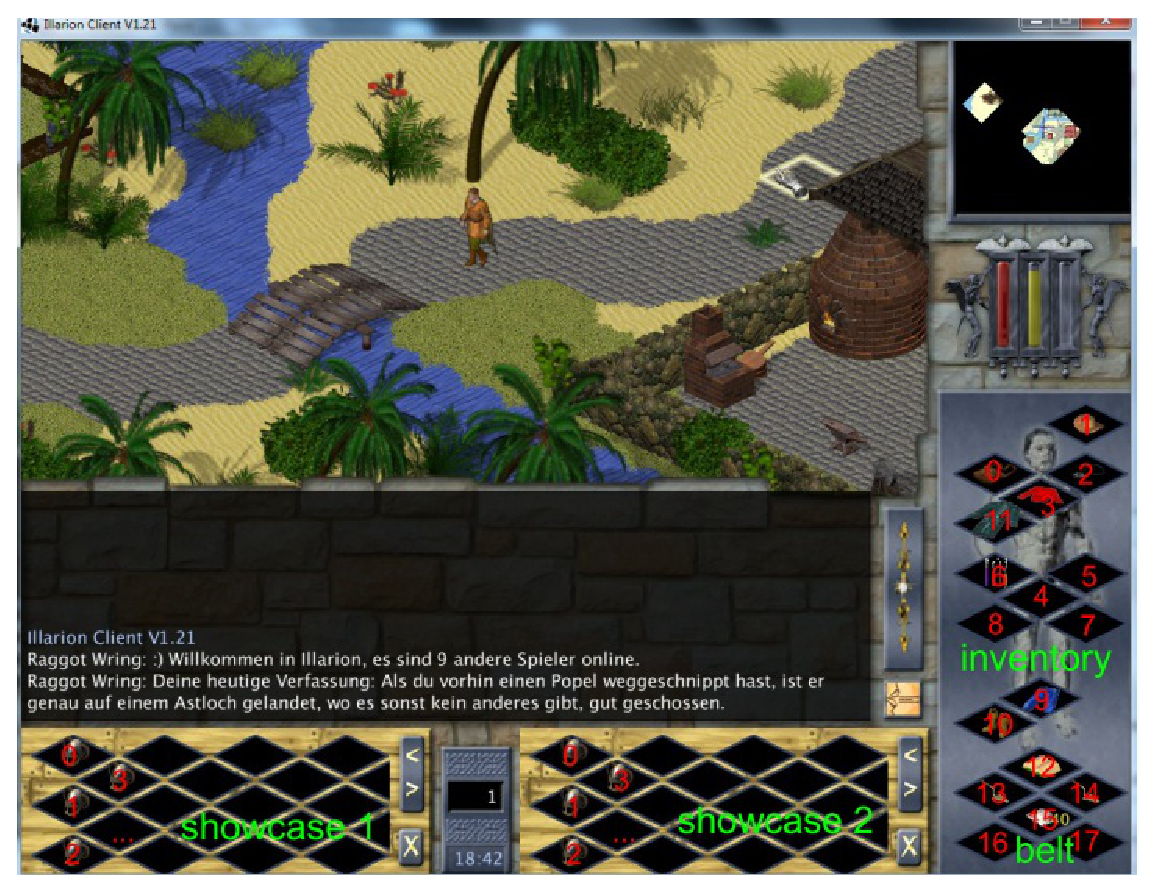
\includegraphics[scale=.8]{itempos.eps}
\end{center}
\caption{Illustration for positions of items. {\color{red}Red: \comm{itempos}}, {\color{green}{Green: \comm{getType}}}}\label{itemtypes}
\end{figure}
\section{Variables}
\lua{r}: \character \var{Item}.\comm{owner}
\begin{quote}
       has the type of \var{character}.
\end{quote}
\lua{r}: \position \var{Item}.\comm{pos}
\begin{quote}
       has the type of \var{position}, this means that the item lies on the floor.
\end{quote}
\lua{r}: \integer \var{Item}.\comm{itempos}
\begin{quote}
       Returns the position of an item if it is at a character.
\end{quote}
\lua{rw}: \integer \var{Item}.\comm{id}
\lua{rw}: \integer \var{Item}.\comm{wear}
\begin{quote}
       Measures how long it will take until the item decays.
\end{quote}
\lua{rw}: \integer \var{Item}.\comm{quality}
\begin{quote}
       The quality of an item is a combination of actual quality (0-9) and durability (0-99).
       A quality of 872 stands for actual quality 8 and durability 72. The item decays shortly after durability hits zero.
       A quality below 100 describes an unfinished item (e.g. for crafting purposes). Quality 64 denotes a 64\% completed item for example.
\end{quote}
\lua{rw}: \integer \var{Item}.\comm{number}
\begin{quote}
       The number of items on that stack.
\end{quote}


\chapter{Items (commonStruct)}
There are unfortunately two types of items. This refers to commonStruct-Items.
Note that there are important functions for items in the chapter "World".
This kind of item variable holds general information about an item (weight, ID,...), not individual ones like, for example, the current position or things like that. It is, so to say, a generalized item.

\section{Variables}
\lua{r}:  \integer \var{Item}.\comm{id}\\
\lua{r}:  \integer \var{Item}.\comm{AgeingSpeed}\\
\lua{r}:  \integer \var{Item}.\comm{Weight}\\
\lua{r}:  \integer \var{Item}.\comm{ObjectAfterRot}\\
\lua{r}:  \integer \var{Item}.\comm{MaxStack}\\
\lua{r}:  \bool \var{Item}.\comm{rotsInInventory}\\
\lua{r}:  \integer \var{Item}.\comm{Brightness}\\
\lua{r}:  \integer \var{Item}.\comm{Worth}\\
\lua{r}:  \txt \var{Item}.\comm{English}\\
\lua{r}:  \txt \var{Item}.\comm{German}\\
\lua{r}:  \txt \var{Item}.\comm{EnglishDescription}\\
\lua{r}:  \txt \var{Item}.\comm{GermanDescription}\\
\lua{r}:  \integer \var{Item}.\comm{Rareness}\\
\begin{quote}
  These variables are accessible for common struct items and script items (where they refer to the corresponding common struct item!).\\
  \emph{Usage}:\\
  \comm{MyItem}.\comm{id}, \comm{MyItem}.\comm{AgeingSpeed}, ...
\end{quote}


\chapter{Weapons and Armor}
\section{WeaponStruct}
\lua{r}:  \integer \var{weaponstruct}.\comm{Attack}\\
\lua{r}:  \integer \var{weaponstruct}.\comm{Defence}\\
\lua{r}:  \integer \var{weaponstruct}.\comm{Accuracy}\\
\lua{r}:  \integer \var{weaponstruct}.\comm{Range}\\
\lua{r}:  \integer \var{weaponstruct}.\comm{WeaponType}\\
\lua{r}:  \integer \var{weaponstruct}.\comm{AmmunitionType}\\
\lua{r}:  \integer \var{weaponstruct}.\comm{ActionPoints}\\
\lua{r}:  \integer \var{weaponstruct}.\comm{MagicDisturbance}\\
\lua{r}:  \integer \var{weaponstruct}.\comm{PoisonStrength}\\
\lua{r}:  \integer \var{weaponstruct}.\comm{Level}\\
\\
WeaponType can be one of the following: WeaponStruct.\{slashing, concussion, puncture, slashingTwoHand, concussionTwoHand, punctureTwoHand, firearm, arrow, bolt, stone, stave, shield\}
\section{ArmorStruct}
\lua{r}:  \integer \var{armorstruct}.\comm{BodyParts}\\
\lua{r}:  \integer \var{armorstruct}.\comm{PunctureArmor}\\
\lua{r}:  \integer \var{armorstruct}.\comm{StrokeArmor}\\
\lua{r}:  \integer \var{armorstruct}.\comm{ThrustArmor}\\
\lua{r}:  \integer \var{armorstruct}.\comm{MagicDisturbance}\\
\lua{r}:  \integer \var{armorstruct}.\comm{Stiffness}\\
\lua{r}:  \integer \var{armorstruct}.\comm{Level}\\
\lua{r}:  \integer \var{armorstruct}.\comm{Type}\\
\\
Type can be one of the following: ArmorStruct.\{clothing, general, light, medium, heavy, jewellery\}
\section{NaturalArmor}
Monsters can have these intrinsic armor properties:\\
\lua{r}:  \integer \var{naturalarmor}.\comm{strokeArmor}\\
\lua{r}:  \integer \var{naturalarmor}.\comm{thrustArmor}\\
\lua{r}:  \integer \var{naturalarmor}.\comm{punctureArmor}\\

\chapter{World}
\section{Functions}
\tile \comm{world}:\com{getField}{\position \var{position}}

\begin{quote}
        \var{position} is a position-structure. The function returns a reference to a field.\\
        Example:
        \begin{verbatim}
            Field=world:getField(position(22,10,-3));   -- get reference to "Field"
            TileID=Field.tile;                          -- Determine the Tile-ID of that field
        \end{verbatim}
\end{quote}
\integer \comm{world}:\com{getTime}{\txt "\var{time}"}
\begin{quote}
  \var{time} can be "year", "month", "day", "hour", "minute", "second" or "unix". The last is the amount of seconds since 1th January 1970 00:00. The others are ingame dates.
\end{quote}
\void \comm{world}:\com{erase}{\scripti \var{Item},\integer \var{amount}}
\begin{quote}
       Example 1:\\
       \comm{world}:\com{erase}{TargetItem,3}\\
       erases 3 items on the TargetItem-Stack if possible\\
       Example 2:\\
       \comm{world}:\com{erase}{TargetItem,0}\\
       erases the whole TargetItem-Stack. (NOTE: Temporarily \emph{DISABLED}!)
       If there are not enough of the items to erase, this function returns "false" and does not delete anything.
\end{quote}
\void \comm{world}:\com{increase}{\scripti \var{Item},\integer \var{count}}
\begin{quote}
       Increases the item number of \var{Item} (\var{SourceItem}, \var{TargetItem}, ...) by \var{count}.
\end{quote}
\void \comm{world}:\com{itemInform}{\character \var{User}, \scripti \var{Item}, \ItemLookAt \var{lookAt}}
\begin{quote}
       Useable in \comm{LookAtItem}: Displays information about an item. ItemLookAt is a class where certain information about the item is stored. An empty instance can be created with lookAt = ItemLookAt(). ItemLookAt has the fields as listed in table \ref{ItemLookAt}. All fields are optional and some of them are coupled with a dedicated item data, storing the corresponding value.

\begin{table}
\begin{tabular}{l|p{3.8cm}|p{3cm}|p{3.5cm}}
    ItemLookAt field & type & item data & description\\ \hline
    name & string & "nameDe"\newline"nameEn"\\
    rareness & ItemLookAt.\newline
        \hspace*{5mm}commonItem\newline
        \hspace*{5mm}uncommonItem\newline
        \hspace*{5mm}rareItem\newline
        \hspace*{5mm}epicItem & "rareness"\\
    description & string & "descriptionDe"\newline"descriptionEn"\\
    craftedBy & string & "craftedBy"\\
    type & string & - & derived from WeaponStruct or ArmorStruct\\
    level & number & - & 0..100\\
    usable & boolean & - & can the player use this?\\
    weight & number & -\\
    worth & number & - & selling price in copper\\
    qualityText & string & -\\
    durabilityText & string & -\\
    durabilityValue & number & - & 0..100 in percent\\
    diamondLevel & number & "magicalDiamond" & magic gem level: 0..10\\
    emeraldLevel & number & "magicalEmerald" & magic gem level: 0..10\\
    rubyLevel & number & "magicalRuby" & magic gem level: 0..10\\
    sapphireLevel & number & "magicalSapphire" & magic gem level: 0..10\\
    amethystLevel & number & "magicalAmethyst" & magic gem level: 0..10\\
    obsidianLevel & number & "magicalObsidian" & magic gem level: 0..10\\
    topazLevel & number & "magicalTopaz" & magic gem level: 0..10\\
    bonus & number & - & gem bonus: 0..255\\
\end{tabular}
\caption{ItemLookAt member variables}\label{ItemLookAt}
\end{table}

\end{quote}
\void \comm{world}:\com{swap}{\scripti \var{Item},\integer \var{newItemID},\integer \var{quality}}
\begin{quote}
  Exchanges \var{Item} (ScriptItem!) with a new one with \var{newItemId} and \var{quality}.
\end{quote}
\scripti \comm{world}:\com{createItemFromId}{\integer \var{ItemID},\integer \var{count},\position \var{position},\bool \var{always-flag},\integer \var{quality},\datatable \var{data}}
\begin{quote}
       where \var{position} is a position-structure and the always-flag is \lua{true} (create also when there is already something on that field) or \lua{false}, depending on how to create the item. It returns a script item sctruct.
\end{quote}
\void \comm{world}:\com{createItemFromItem}{\scripti \var{Item},\position \var{Position},\\var{always-flag}}
\begin{quote}
       where \var{Item} is of the scriptitem-structure. (NOT of the common-structure! Therefore this IS
       usable with TargetItem!). It creates an identical copy of a scriptitem.
\end{quote}
\character \comm{world}:\com{createMonster}{\integer \var{monsterID},\position \var{position},\integer \var{movepoints}}
\begin{quote}
    Summons a monster with the given monster-ID at the given location. For a list of monster-IDs, please consult the database or a fellow developer.
\end{quote}
\character \comm{world}:\com{createDynamicNPC}{\txt \var{name}, \integer \var{race}, \position \var{position}, \integer \var{sex}, \txt \var{scriptname}}
\begin{quote}
    Summons an NPC with the given parameters, using the script that is stated.
\end{quote}
\textsl{list} \comm{world}:\com{LoS}{\position \var{start position}, \position \var{end position}}
\begin{quote}
    Returns a list that contains lists that contain the type of the list entry and the corresponding items and characters that block the way between \var{start position} and \var{end position} and is \lua{nil} otherwise. They can easily be referenced by e.g. \texttt{list[1].TYPE}, which returns either \texttt{"ITEM"} or \texttt{"CHARACTER"} and \texttt{list[1].OBJECT} which contains either the item-struct or the character-struct. For the following example, imagine that an item with the item-ID 100 and after that, a character with the character-ID 666 block the way between \texttt{startPos} and \texttt{endPos}:
    \begin{verbatim}
        ...
        list=world:LoS(startPos, endPos);
        if (list ~= nil) then
            for key, listEntry in pairs(list) do
                if (listEntry.TYPE == "ITEM") then
                    User:inform("Item with the ID: "..listEntry.OBJECT.id);
                elseif (listEntry.TYPE == "CHARACTER") then
                    User:inform("Character with the ID: "..listEntry.OBJECT.id);
                end
            end
        else
            User:inform("Nothing blocks the way!");
        end
        ...
    \end{verbatim}
    This will produce the output:
    \begin{verbatim}
    Item with the ID: 100
    Character with the ID: 666
    \end{verbatim}
\end{quote}
\void \comm{world}:\com{makeSound}{\integer \var{Number},\position \var{position}}

\begin{quote}
       Starts soundeffect.
       1=scream, 2=sheep, 3=sword hit, 4=thunder, 5=bang, 6=chopping wood, 7=fire, 8=smithing, 9=water splash, 10=pouring in (bottle), 11=saw, 12=drink, swallow, 13=snaring noise
\end{quote}
\void \comm{world}:\com{gfx}{\integer \var{Number},\position \var{position}}

\begin{quote}
       Starts graphicseffect on \var{position}.
\end{quote}
\void \comm{world}:\com{changeTile}{\integer \var{TileID},\position \var{position}}\\
\commoni \comm{world}:\com{getItemStats}{\scripti \var{Item}}
\begin{quote}
       Returns an commonitem-struct from an \var{Item} that is a scriptitem (like TargetItem).
       Example:\\
       \begin{verbatim}
       myItem=world:getItemStats(TargetItem)
       if (myItem.Weight<100) then
           ...
       end
       \end{verbatim}
\end{quote}
\commoni \comm{world}:\com{getItemStatsFromId}{\integer \var{ItemID}}
\begin{quote}
       Returns an item-struct like \comm{world}:\com{getItemStats}{\var{Item}}
\end{quote}
\scripti \comm{world}:\com{getItemOnField}{\position \var{Position}}
\begin{quote}
       Returns a scriptItem on that field.
\end{quote}
\bool \comm{world}:\com{isItemOnField}{\position \var{Position}}\\
\bool \comm{world}:\com{isCharacterOnField}{\position \var{Position}}
\begin{quote}
       Returns \lua{true} for a Character standing on that position and \lua{false} otherwise.
\end{quote}
\character \comm{world}:\com{getCharacterOnField}{\position \var{Position}}
\begin{quote}
       Returns a character-struct. See chapter "Characters".
       Example:
\begin{verbatim}
  ...
  myPosition=position(122,12,3);
  if world:isCharacterOnField(myPosition) then
      myPerson=world:getCharacterOnField(myPosition);
      myPerson:talk(Character.say,"You found me!");
  end
  ...
  \end{verbatim}
\end{quote}
\character \comm{world}:\com{getPlayersInRangeOf}{\position \var{Position}, \integer \var{Range}}
\begin{quote}
       Returns a list of character-structs who are in the \var{Range} of \var{Position}. See chapter "Characters" and lists in lua.
\end{quote}
\character \comm{world}:\com{getCharactersInRangeOf}{\position \var{Position}, \integer \var{Range}}
\\
\character \comm{world}:\com{getNPCSInRangeOf}{\position \var{Position}, \integer \var{Range}}
\\
\character \comm{world}:\com{getMonstersInRangeOf}{\position \var{Position}, \integer \var{Range}}
\\
\character \comm{world}:\com{getPlayersOnline}{}
\begin{quote}
       Returns a list of character-structs of all players online. See chapter "Characters" and lists in lua.
\end{quote}
\void \comm{world}:\com{changeQuality}{\scripti \var{ScriptItem},\integer \var{amount}}
\begin{quote}
       Changes the quality of a scriptitem (TargetItem, ...) for \var{amount}.
\end{quote}
\void \comm{world}:\com{changeTile}{\integer \var{tileid},\position \var{position}}
\begin{quote}
       Changes the tile on position-struct "position" to tileid. To be combined with the following command.
\end{quote}
\void \comm{world}:\com{sendMapUpdate}{\position \var{position},\integer \var{range}}
\begin{quote}
       Send a map update to all clients of characters that stand in range of that position.
\end{quote}
\txt \comm{world}:\com{getItemName}{\integer \var{Itemid},\integer \var{PlayerLanguage}}
\begin{quote}
       Returns string that represents the itemname of the item with this id in playerlanguage according to table "itemnames".
\end{quote}
\void \comm{world}:\com{changeItem}{\scripti \var{ScriptItem}}
\begin{quote}
       Changes a scriptitem against a new one. Handle with care!
       Example:
       \begin{verbatim}
  function UseItem(User, SourceItem)
        SourceItem.id = 1               -- we change the source Item to a sword
        SourceItem.quality = 699        -- a really good sword.
        SourceItem.wear = 10            -- a sword wich rots in a very long time
        world:changeItem(SourceItem)    -- now the item is changed
  end
  \end{verbatim}
\end{quote}
\bool , \weapon \comm{world}:\com{getWeaponStruct}{\integer \var{itemID}}
\begin{quote}
        Returns two values: bool (true if it is a weapon) and the weaponstruct of the given item (if there is any).\\
        \emph{Example}:
        \begin{verbatim}
            ...
            foundWp,MyWeapon=world:getWeaponStruct(1);
            if (foundWp==true) then
                User:inform("Attack: " .. MyWeapon.Attack .. " def: " .. MyWeapon.Defence);
            end
            ...
        \end{verbatim}
\end{quote}
\bool , \armor \comm{world}:\com{getArmorStruct}{\integer \var{itemID}}
\begin{quote}
       Returns two values: bool (true if it is an armor) and the armorstruct of the given item.
\end{quote}
\bool , \naturalarmor \comm{world}:\com{getNaturalArmor}{\integer \var{raceID}}
\begin{quote}
       Returns two values: bool (true if that race has natural armor) and the naturalarmorstruct of the given race.
\end{quote}

\section{Variables}
\lua{r,w}: \textsl{weatherStruct} \comm{weather}
\begin{quote}
    Returns the current weather.
\end{quote}

\chapter{Fields}
\section{Functions}
In general, these functions will be combined with \comm{world}:\com{getField}{\position \var{position}} most of the time.\\
\void \var{field}:\com{swapTopItem}{\integer \var{newId}, \integer \var{quality}}
\\
\integer \var{field}:\com{countItems}{}
\begin{quote}
    Returns the number of items that are placed on top of that field.
\end{quote}
\scripti \var{field}:\com{getStackItem}{\var{stackpos}}
\begin{quote}
    Returns the item with position \var{stackpos} (0 being the bottom item) within the pile of items on this field. If \var{stackpos}
    exceeds the number of items on that field, a 0-item is returned (id=0), therefore it is a good idea to check the number of items on that field first.
\end{quote}

\begin{quote}
       Changes the top item on a field to newId with quality. 0 to let the quality unchanged.
\end{quote}
\void \var{field}:\com{changeQualityOfTopItem}{\integer \var{amount}}
\begin{quote}
       An easy way to change the quality of that item which the player would pick up.
\end{quote}
\bool \var{field}:\com{isPassable}{}
\begin{quote}
       Determines whether a field allows a character to pass over it or having items dropped on it.
\end{quote}

\section{Variables}
\lua{r}: \integer \comm{tile}
\begin{quote}
    Returns the tile ID of that field. Recommended use with \comm{world}:\com{getField}{\var{position}}.
\end{quote}


\chapter{It's a kind of magic}
\section{Global variables}
\comm{thisSpell}
\begin{quote}
       Refers to the ID of the spell that is currently casted.
\end{quote}
\section{Some words on magic}
Casting a spell is done by selecting one or more \index{runes}runes and eventually selecting a target. We assign numbers to these runes like in fig(\ref{runes}).
\begin{figure}[htp]
\begin{center}
\includegraphics[scale=.5]{runes.eps}
\end{center}
\caption{The runes}\label{runes}
\end{figure}
Every spell gets a unique spell-ID which is entirely determined by the used runes. Suppose we have to use the runes with the numbers $a_1 \dots a_n$ to cast that spell, the spellId can then be calculated by
\begin{equation}
  I_{\mathrm{spell}}=\sum_{k=1}^n 2^{a_k-1}=2^{a_1-1}+2^{a_2-1}+\cdots+2^{a_n-1}.
\end{equation}
To give a concrete example: Imagine for your spell you have to use runes 2 and 5. The spell Id then is
\begin{equation}
  I_{\mathrm{spell}}=\sum_{k=1}^2 2^{a_k-1}=2^{a_1-1}+2^{a_2-1}=2^{2-1}+2^{5-1}=2^1+2^4=2+16=17.
\end{equation}
The caption of every spell script should include a brief description of the spell, the rune combination and the SQL insert statement (as comments, of course):\\
   \comm{INSERT INTO spells VALUES}(\var{spellID},\var{magicType},`\var{scriptname.lua}`)\\
In our case, that might be: \verb"INSERT INTO spells VALUES(17,0,'m_17_fireball.lua')"

\chapter{Weather}
Till now, weather is a global effect. Once you set the weather to a specific value, it's the same everywhere. Eventually
there will be "areas" of weather in the future. A weatherStruct is a set of different variables, just like any other struct
so far. Altering these variables changes the weather.
\section{Variables}
\lua{rw}: \integer \var{weatherStruct}.\comm{cloud\_density}
\begin{quote}
  Varies between 0 (no clouds) and 100 (full clouds).
\end{quote}
\lua{rw}: \integer \var{weatherStruct}.\comm{fog\_density}\\
\lua{rw}: \integer \var{weatherStruct}.\comm{wind\_dir}\\
\lua{rw}: \integer \var{weatherStruct}.\comm{gust\_strength}\\
\lua{rw}: \integer \var{weatherStruct}.\comm{percipitation\_strength}\\
\lua{rw}: \integer \var{weatherStruct}.\comm{percipitation\_type}\\
\lua{rw}: \integer \var{weatherStruct}.\comm{thunderstorm}\\
\lua{rw}: \integer \var{weatherStruct}.\comm{temperature}\\

\section{Functions}


\section{Entry point}
There is just one entry point for weather scripts:
\lua{function} \com{changeWeather}{}
\begin{quote}
       Is invoked everytime the weather should be changed.
\end{quote}

\chapter{Long time effects}
\section{Basic idea}
Long time effects (LTEs) allow you to influence a character over a period of time. The values are saved in the database, so they endure even a server crash.

LTEs are bound to a character. They basically consist of:
\begin{itemize}
\item The name (only visible in the database) and the ID of the LTE
\item A script that defines the LTE
\item A counter that counts how often an effect had been called already
\item A variable that controls when this effect on this character will be called again
\item Several self defined variables that can be accessed by a key string and that can hold an integer.
\end{itemize}

First, one has to add the LTE to the database with a unique ID, a name and a script name, e.g. {\tt 42} is the ID, {\tt myeffect} the name and {\tt myeffect.lua} the script.

Then one has to add the effect to a character, e.g. inside an item script. How the effect works has to be defined in its script {\tt myeffect.lua}. Everytime the LTE is called, its script is invoked; to be exact, the function \comm{callEffect} is invoked, see the section about Entry Points. There one can change the character's attributes etc. Note that you should always save any change of fixed attributes as a value of the LTE, so you can restore everything when the LTE ends.

If the character logs out, all values are saved. If he logs in again, the function \comm{loadEffect} in the LTE script is invoked. Any temporary change of attributes will be gone by now, so here you can read the value you have saved and do the change again.

The example at the end of this chapter will help you a lot.

\section{Functions}
\void \var{effect}:\com{addValue}{\txt \var{name},\integer \var{value}}
\begin{quote}
       \var{name} is an arbitrary name for a variable that can be introduced and filled with \var{value} and is added
       to that effect. It can later (at one of the following calls, for example) be read or changed again. Note that \var{value} can be any integer x, but it will be saved as y, where $0 \le y < 2^{32}$ and $x \equiv y \pmod{2^{32}}$.
\end{quote}
\void \var{effect}:\com{removeValue}{\txt \var{name}}
\begin{quote}
       \var{name} is the name of a value that will be removed from that effect.
\end{quote}
\bool , \integer \var{effect}:\com{findValue}{\txt \var{name}}
\begin{quote}
       This function returns {\tt true} if a value \var{name} is found plus its value and {\tt false} otherwise. Note that these are two values!
\end{quote}
\bool, \effect  \var{Character}.\comm{effects}:\com{find}{\var{effect-ID}}
\begin{quote}
		This function returns {\tt true} if an effect with \var{effect-ID} was
		found and the respective \var{effect}, {\tt false} otherwise.
\end{quote}
\void \var{Character}.\comm{effects}:\com{addEffect}{\com{LongTimeEffect}{\var{effect-ID},\integer \var{nextCalled}}}
\begin{quote}
This function adds the effect \var{effect-ID} to a character. One also has to set the initial \var{nextCalled} value. Thus, right after the script, which contains this command, is completely executed, the function \comm{addEffect} in the effect's script is called and, if not changed in \comm{addEffect}, the function \comm{callEffect} is called after \var{nextCalled}$\cdotp \frac{1}{10}$ seconds.
\end{quote}
\bool \var{Character}.\comm{effects}:\com{removeEffect}{\var{effect-ID}}
\begin{quote}
       This function removes the effect \var{effect-ID} from a character. It returns a boolean which indicates whether that worked or not.
\end{quote}

\section{Variables}
\lua{r}:  \integer \var{effect}.\comm{effectId}\\
\lua{r}:  \integer \var{effect}.\comm{effectName}\\
\lua{r,w}:  \integer \var{effect}.\comm{nextCalled}

\emph{IMPORTANT:} \comm{nextCalled} must not exceed $2^{31}-1$, otherwise the effect won't be safed properly.\\
\lua{r}:  \integer \var{effect}.\comm{lastCalled}\\
\lua{r}:  \integer \var{effect}.\comm{numberCalled}\\


\section{Entry points for longtime effects}
Inside that script which was invoked, there are several possible entry points that can be called:\\
\lua{function} \com{callEffect}{\var{Effect}, \var{Character}}
\begin{quote}
       MUST either return {\tt true} if the effect should be called again or {\tt false} if not! \var{Effect}.\comm{nextCalled} has to be set. It will be lowered by 1 every $\frac 1 {10^{\mathrm {th}}}$ second and \comm{callEffect} will be called as soon as it reaches $0$.
\end{quote}
\lua{function} \com{addEffect}{\var{Effect}, \var{Character}}
\begin{quote}
       Is invoked when an effect is newly created.
\end{quote}
\lua{function} \com{removeEffect}{\var{Effect}, \var{Character}}
\begin{quote}
       Is invoked after an effect ended (by having \comm{callEffect} return {\tt false}.
\end{quote}
\lua{function} \com{doubleEffect}{\var{Effect}, \var{Character}}
\begin{quote}
       Is invoked when an effect is added to a character that already has that effect. Note that a character can hold just one effect of one type at a time! \\
This function is currently bugged, as all effect values are deleted when the effect is re-added (see Mantis issue \#451).
\end{quote}
\lua{function} \com{loadEffect}{\var{Effect}, \var{Character}}
\begin{quote}
       Is invoked when a player character logs into the game. It should be used to set temporary stats changes and so on, which can be stored in effect-variables, using \comm{findValue} and so on.
\end{quote}

\section{Example: Adding long time effects to characters}
Imagine the following situation: You drink a potion of a fluid and after that, you get "drunk", that means that your perception and agility are lowered and you sometimes make uncontrolled steps for the next 4 minutes.
The first thing to do is to create a table entry in {\tt longtimeeffects} in the following way:
\begin{verbatim}
 lte_effectid | lte_effectname | lte_scriptname
--------------+----------------+-----------------
          666 | alcohol        | lte_alcohol.lua
\end{verbatim}
To start with, we need to script the bottle ({\tt bottle.lua}) which adds the effect 666 ({\tt alcohol}) to the character drinking that bottle.
%\begin{boxedminipage}[h]{4cm}
%\begin{lstlisting}[numbers=left, frame=shadowbox, caption=test]
\begin{verbatim}
function UseItem(User, SourceItem, LTstate)

    foundEffect, alcEffect = User.effects:find(666); -- does effect #666 already exist?

    if (not foundEffect) then              -- if that effect is not there...
        alcEffect = LongTimeEffect(666,10); -- create new effect
        User.effects:addEffect(alcEffect);    -- add effect #666
                            -- funct. "addEffect(...)" in the LT-script will be called.
                            -- 1 second until first call of "callEffect(...)"
        foundEffect = User.effects:find(666);   -- does effect #666 exist now?
        if (not foundEffect) then              -- effect not found (security check)
            User:inform("An error occured, inform a developer.");
            return;                             -- exit immediately if not found!
        end
    end

    alcEffect:addValue("alcLevel",10);      -- sets the alcLevel-value to 10.
    alcEffect:addValue("strMod",-5);        -- sets modifier for strength to -5.

end
\end{verbatim}
%\end{lstlisting}
%\end{boxedminipage}
So, this script simply adds {\tt alcEffect} (666) to the {\tt User} of the bottle and adds the value {\tt alcLevel} to this effect and sets it to 10.

The next thing to be done is to define this effect. This is done in the actual long time script we defined in the database before, {\tt lte\_alcohol.lua}:
\begin{verbatim}
function addEffect(myEffect, Character)     -- called only the first time
    Character:inform("You feel a little bit dizzy.");
    found, strMod = myEffect:findValue("strMod");
    if found then                           -- read the str modificator
        Character:increaseAttrib("strength",strMod);
    else                                    -- if modificator is not found
        Character:inform("Error, please inform a developer");
        myEffect:addValue("strMod",-5);     -- set to a default value
    end
end

function callEffect(myEffect, Character)    -- is called everytime
    found, alcLevel = myEffect:findValue("alcLevel");
                                            -- get value
    Character:talk(Character.say,"Hick!"); -- Hick!
        -- add some more effects
    if not found then
        Character:inform("Error, please inform a developer!")
        return false;                       -- bug occured! remove effect
    else
        if (alcLevel>0) then                -- alcohol still has effect
            myEffect.nextCalled=200;        -- next call in 20 s.
            myEffect:addValue("alcLevel",alcLevel-1);
                                            -- just override the value
            return true;
        else                                -- alcohol has no more effect
            myEffect:removeValue("alcLevel");
            return false;                   -- return false and remove effect
        end
    end
end

function loadEffect(myEffect, Character)    -- is called when the character logs in
                                            -- do the STR change again
    Character:inform("You still feel a little bit dizzy.");
    found, strMod = myEffect:findValue("strMod");
    if found then                           -- read the str modificator
        Character:increaseAttrib("strength",strMod);
    else                                    -- if modificator is not found
        Character:inform("Error, please inform a developer");
        myEffect:addValue("strMod",-5);     -- set to a default value
    end
end
\end{verbatim}

\section{Ideas for usage}
Long time effects can be used for many effects, here are just some ideas:
\begin{itemize}
\item Illness, epidemy, infections and deseases
\item Injuries
\item Effects of potions (of all kinds)
\item Effects of poison
\item Punishment
\item \dots
\end{itemize}

\chapter{Delayed execution and disturbation}
There is a way to have a script being executed after some time. Of course, this could also be done using long time effects,
which were described above. However, there is something that long time effects can't detect: If "something" happened between
two invokations of an effect. Take, for example, a magician who casts a spell. Assume that there is a delay between casting
that spell and having an effect (it needs some time of concentration). What happens if, for example, this mage is disturbed
during the concentration phase (because he's under attack or alike)? There is no way to detect that in long time effect scripts.

\section{Functions}
\void \var{Character}:\com{startAction}{\integer\var{time}, \integer\var{GFX-ID}, \integer\var{GFX-interval}, \integer\var{SFX-ID}, \integer\var{SFX-interval}}
\begin{quote}
This starts an action for the character for \var{time} $\frac{1}{10th}$seconds. The GFX with ID \var{GFX-ID} is shown every \var{GFX-interval} $\frac{1}{10th}$seconds. The SFX with ID \var{SFX-ID} is played every \var{SFX-interval} $\frac{1}{10th}$seconds.
\end{quote}
\void \var{Character}:\com{changeSource}{\character \var{item}}\\
\void \var{Character}:\com{changeSource}{\scripti \var{item}}\\
\void \var{Character}:\com{changeSource}{\position \var{position}}
\begin{quote}
Changes the source variable of the entrypoint used for subsequent calls of the current action. This has to be called explicitly to propagate changes of a source object to the action.
\end{quote}

\section{Constants}
\integer \comm{Action.none} \\
\integer \comm{Action.abort}

\section{Usage}
In all "Use"-functions like \com{UseItem}{...}, the last parameter is the integer \var{ltstate}. Its value is one of the constants above. So one can check the \var{ltstate} and eventually start an action.

There can only be one action at a time for a character. If multiple actions are started in the same script, only the last one counts (nevertheless the "first" sound is played and the "first" gfx is shown for every action immediately, if the interval is greater than 0).

After starting an action, the script is still executed until its end. Then after the \var{time} OR if the character got interrupted (was attacked, moved, used something...), the script is called again and is normally executed. So make sure to check the \var{ltstate}!

\section{Example}
A simple example of a potion script is helpful:

\begin{verbatim}
function UseItem(User, SourceItem, ltstate)

    -- check for ltstate == Action.abort
    -- means the script got interrupted before the time needed was up
    -- (-> drinking was not finished!)
    if (ltstate == Action.abort) then

        -- Cast forced emotes from the Charakter who uses our potion
        -- (german for germans, english for the rest)
        User:talk(Character.say, "#me verschüttet den Trank.", "#me spills the potion.")
        -- [...] possibly remove the bottle etc.
        -- since the user failed to drink the potion we are done now
        return
    end

    -- [...] possibly check if the character is in attackmode

    -- Now we check if the character is drinking the potion currently or not
    -- (since the drinking process needs some time)
    if (ltstate == Action.none) then
        -- Action.none so the character does nothing.
        -- Lets open the bottle and drink the potion

        -- Start the action!
        -- 2,0 seconds until the action is done
        -- GFX id 0 is shown while the waiting time ( so no gfx )
        -- every 0 seconds the GFX is shown ( so never )
        -- SFX id 15 is played ( drinking sound )
        -- every 2,5 seconds. So the sound is only played once (at the beginning)
        User:startAction(20,0,0,15,25);

        -- let's tell everyone that our user drank a potion with a forced emote
        User:talk(Character.say, "#me beginnt einen Trank zu trinken.", "#me starts to trink a potion.")

        -- And quit the script since we are done now and waiting for the next call
        return
    end

    -- since we are here the character started already to drink
    -- but got not interrupted. Now we offer some results

    -- [...] possibly remove the bottle, give healthpoints and foodpoints
    -- and slow down the character
    -- [...] etc.

end
\end{verbatim}

\chapter{Waypoints}
The waypoint system allows us to use the pathfinding algorithm of the server for moving monsters and NPCs through the terrain. There is an internal list of position data which is handled like a queue, so first in - first out. The character always tries to reach the first waypoint, until the list is empty.

The algorithm checks for obstacles and a free way only in a certain radius. This process is quite expensive (and even more important: the server freezes until the algorithm finishes!), so the radius shouldn't be too big; around 15 tiles should suffice (the default value is currently unknown, but it won't be much more).
\section{Functions}
The waypoint list can be accessed by \var{character}.\comm{waypoints} and the following operations are possible:
\\\\
\void \var{character}.\comm{waypoints}:\com{addFromList}{\var{waypointlist}}
\begin{quote}
Adds a whole Lua list of position structs to the end of the internal list.
\end{quote}
\void \var{character}.\comm{waypoints}:\com{addWaypoint}{\var{pos}}
\begin{quote}
Adds a single position struct \var{pos} as last waypoint to the internal list.
\end{quote}
\lualist{ \position} \var{character}.\comm{waypoints}:\com{getWaypoints}{}
\begin{quote}
Returns the internal list as Lua list of position structs.
\end{quote}
\void \var{character}.\comm{waypoints}:\com{clear}{}
\begin{quote}
Clears the internal list.
\end{quote}

For controling the character there are these functions:
\\\\
\void \var{character}:\com{setOnRoute}{\bool \var{toggleRoute}}
\begin{quote}
The character starts the route if \var{toggleRoute} is \lua{true} and stops if it is \lua{false}.
\end{quote}
\bool \var{character}:\com{getOnRoute}{}
\begin{quote}
Returns if the character is currently on a route.
\end{quote}
\bool, \integer \var{character}:\com{getNextStepDir}{\position \var{pos}, \integer \var{rangeToCheck}}
\begin{quote}
Returns two values. The first is \lua{true} if a way to \var{pos} is found considering only a radius of \var{rangeToCheck} tiles, \lua{false} otherwise. The second is the direction of the next step for the found way.

This function does not move the character, it just returns the direction for the next step.
\end{quote}
\lualist{\integer} \var{character}:\com{getStepList}{\position \var{pos}, \integer \var{rangeToCheck}}
\begin{quote}
Same as \com{getNextStepDir} but returns a complete step list to reach \var{pos}.
\end{quote}

\section{Entry Points}
If a character (Monster/NPC) is on a route, no other handling inside the server is done (no fighting) but all the script entry points like enemyNear or enemyInSight are called.

There is one special entry point for both monsters and NPCs: \\
\lua{function} \com{abortRoute}{\var{character}}
\begin{quote}
Is called if the \var{character} has reached the destination or if items block the way and the destination can't be reached.
\end{quote}

\chapter{Global Scriptvariables}
These ScriptVars allow us to save a value in the database and access it by an identifier string. Use with caution as they have global effect. All ScriptVars are automatically saved upon a server shutdown.

\section{Functions}
\void \com{ScriptVars:set}{\var{identifier}, \var{value}}
\begin{quote}
Writes the integer or string \var{value} to the ScriptVar \var{identifier}.
\end{quote}
\bool, \var{value} \com{ScriptVars:find}{\var{identifier}}
\begin{quote}
Returns if there exists a ScriptVar \var{identifier}. If \lua{true} then its \var{value} is returned aswell.
\end{quote}
\bool \com{ScriptVars:remove}{\var{identifier}}
\begin{quote}
Removes the ScriptVar \var{identifier}, returns \lua{true} if there was such a value.
\end{quote}
\void \com{ScriptVars:save}{}
\begin{quote}
Saves all ScriptVars immediately. Use with caution as it could cause freezes.
\end{quote}

\chapter{Random}
Most of the time the random number generator supplied by Lua should be enough. However, if you are looking for a statistically sound implementation of a random number generator, or need another distribution besides the uniform one, this is the class you are looking for.

\section{Functions}
\double \com{Random.uniform}{}
\begin{quote}
       Returns a random floating-point value uniformly distributed in the range [0..1).
\end{quote}
\integer \com{Random.uniform}{\integer \var{min}, \integer \var{max}}
\begin{quote}
       Returns a random integer value uniformly distributed in the range [\var{min}..\var{max}].
\end{quote}
\double \com{Random.normal}{\double \var{mean}, \double \var{standard\_deviation}}
\begin{quote}
       Returns a random floating-point value normally distributed with given \var{mean} and \var{standard\_deviation}.
\end{quote}

\chapter{Debugging}
While using luac -p for finding compilation errors is very straight forward, it is much more difficult to find runtime errors. The script error log which can be viewed via \url{http://illarion.org/~nitram/show_log.php} for the testserver and via \url{http://illarion.org/~vilarion/show_log.php} for the illarionserver shows all runtime errors and where they occured. These logs should be checked after every change and subsequent testing. Keeping the logs clean will help others to find their own bugs faster.

\section{Functions}
\void \com{debug}{\txt \var{debugMessage}}
\begin{quote}
       If used on the testserver prints \var{debugMessage} to the script log together with a stacktrace showing where the call of \com{debug}{...} originated. Has no effect on the illarionserver.
\end{quote}

\chapter{Entry Points}

\section{Items}

\lua{function} \com{UseItem}{\var{User}, \var{SourceItem}, \var{ltstate}}
\begin{quote}
When one item is used. If it is used with another item, \var{TargetItem} is the ID of that item, otherwise it is 0.
\end{quote}
\lua{function} \com{LookAtItem}{\var{User}, \var{Item}}
\begin{quote}
       When someone looks at an item.
\end{quote}
\lua{function} \com{MoveItemBeforeMove}{\var{User}, \var{SourceItem}, \var{TargetItem}}
\begin{quote}
       Is invoked when someone tries to move an item before the move is commited.
       If this function returns \lua{false} the move of the item will not be carried out; that can be used for cursed items.\\
       Basically, \var{SourceItem} is the item before it was moved, \var{TargetItem} is the item after it was moved.\\
       \comm{IMPORTANT:} It MUST return either \lua{true} or \lua{false}, otherwise the server crashes! ( \lua{return true;})
\end{quote}
\lua{function} \com{MoveItemAfterMove}{\var{User}, \var{SourceItem}, \var{TargetItem}}
\begin{quote}
       Is invoked after someone moved an item. See also \com{MoveItemBeforeMove}.
\end{quote}
\lua{function} \com{NextCycle}{}
\begin{quote}
       Is invoked every 10 seconds for commonitems.
\end{quote}
\lua{function} \com{CharacterOnField}{\var{User}}
\begin{quote}
       Is invoked if someone steps on that item (which therefore lies on the floor); good for traps and fields.
       This function requires that the corresponding item has a specialitem-flag in the db-table tilesmodificators
\end{quote}

\section{NPC}
For effective usage of NPCs and their scripts please read the section about string handling.\\
\lua{function} \com{nextCycle}{\var{npc}}
\begin{quote}
       Is invoked every few server cycles (=approximately constant time intervalls, $\frac{1}{10}$s). \emph{IMPORTANT:} MUST exist in NPC scripts!
\end{quote}
\lua{function} \com{receiveText}{\var{npc}, \var{TextTyp}, \var{Text}, \var{Originator}}
\begin{quote}
       Is invoked if the NPC hears someone speaking (even himself!).
\end{quote}
\lua{function} \com{useNPC}{\var{npc}, \var{User}}
\begin{quote}
       Is invoked if the NPC is used (shift-click) by \var{User} without target.
\end{quote}
\lua{function} \com{lookAtNpc}{\var{npc}, \var{SourceCharacter}, \var{mode}}
\begin{quote}
Is invoked if the player \var{SourceCharacter} looks at the NPC. \var{mode} describes what kind of lookat is done: 0 means normal, 1 means close examination.
\end{quote}

\section{Magic}
\lua{function} \com{CastMagic}{\var{Caster}}
\begin{quote}
       Is invoked when \var{Caster} casts a spell without target.
\end{quote}
\lua{function} \com{CastMagicOnCharacter}{\var{Caster}, \var{TargetCharacter}}
\begin{quote}
       Is invoked when \var{Caster} casts a spell on another character/monster (\var{TargetCharacter}).
\end{quote}
\lua{function} \com{CastMagicOnField}{\var{Caster}, \var{pos}}
\begin{quote}
       Is invoked when \var{Caster} casts a spell on a field at the position \var{pos}.
\end{quote}
\lua{function} \com{CastMagicOnItem}{\var{Caster}, \var{TargetItem}}
\begin{quote}
       Is invoked when a spell is casted on an item.
\end{quote}

\section{Monsters}

\lua{function} \com{onDeath}{\var{Monster}}
\begin{quote}
       Is invoked as a monster dies.
\end{quote}
\lua{function} \com{receiveText}{\var{Monster}, \var{TextTyp}, \var{Text}, \var{Originator}}
\begin{quote}
       Is invoked when a monster (\var{Monster}) receives spoken text.
\end{quote}
\lua{function} \com{onAttacked}{\var{Monster}, \var{Attacker}}
\begin{quote}
       Is invoked when a monster is attacked.
\end{quote}
\lua{function} \com{onCasted}{\var{Monster}, \var{Caster}}
\begin{quote}
       Is invoked when a spell is casted on a monster.
\end{quote}
\lua{function} \com{useMonster}{\var{Monster}, \var{User}}
\begin{quote}
       Is invoked when a monster is used by \var{User}
\end{quote}
\lua{function} \com{onAttack}{\var{Monster},\var{Enemy}}
\begin{quote}
       Is invoked every time when a monster would hit the enemy.
\end{quote}
\lua{function} \com{enemyOnSight}{\var{Monster},\var{Enemy}}
\begin{quote}
       Is invoked every time when a monster sees an enemy. \emph{IMPORTANT}: MUST return true (did something) or false (did nothing)!
       It is not invoked when the monster stands on a field next to the enemy.
\end{quote}
\lua{function} \com{enemyNear}{\var{Monster},\var{Enemy}}
\begin{quote}
       Is invoked every time when a monster sees an enemy and stands next to it. Works exactly like \com{enemyOnSight}, MUST return true or false! But beware: If you plan to have \com{setTarget}{...} return 0 ("don't attack anyone"), \com{enemyNear}{...} must return false, otherwise the server is caught in an endless loop!
\end{quote}
\lua{function} \com{lookAtMonster}{\var{SourceCharacter}, \var{monster}, \var{mode}}
\begin{quote}
Is invoked if the player \var{SourceCharacter} looks at the \var{monster}. \var{mode} describes what kind of lookat is done: 0 means normal, 1 means close examination.
\end{quote}
\lua{function} \com{onSpawn}{\var{Monster}}
\begin{quote}
Is called immediately after the \var{Monster} has spawned. There one can e.g. set it on a route using waypoints.
\end{quote}
\lua{function} \com{setTarget}{\var{Monster}, \var{CandidateList}}
\begin{quote}
If setTarget exists, it is called whenever \var{Monster} need to decide what it should attack. \var{CandidateList} is a list of players who are possible targets. To set a target, it's index in that list has to be returned. The first enemy in the list has the index 1. If the function returns 0, the monster will ignore any enemy. If \com{setTarget}{} returns 0 ("don't attack anyone"), \com{enemyNear}{} must return false otherwise the server is caught in an endless loop!

If setTarget does not exist, the player with lowest health is chosen by default.
\end{quote}

\section{Fields}

\lua{function} \com{useTile}{\var{User},\var{Position}}
\begin{quote}
       Is invoked when a tile is shift-clicked (used).
\end{quote}
\lua{function} \com{MoveToField}{\var{User}}
\begin{quote}
       Is invoked if a character moves on that triggerfield (entry in "triggerfields" necessary).
\end{quote}
\lua{function} \com{MoveFromField}{\var{User}}
\begin{quote}
       Is invoked if a character moves away from that triggerfield.
\end{quote}
\lua{function} \com{PutItemOnField}{\var{Item},\var{User}}
\begin{quote}
       Is invoked if an item is put on that triggerfield.
\end{quote}
\lua{function} \com{TakeItemFromField}{\var{Item},\var{User}}
\begin{quote}
       Is invoked if an item is taken away from that triggerfield.
\end{quote}
\lua{function} \com{ItemRotsOnField}{\var{oldItem},\var{newItem}}
\begin{quote}
       Is invoked when \var{oldItem} rots into \var{newItem} on a triggerfield.
\end{quote}

\section{Quests}
While you can create quests with setQuestProgress and getQuestProgress, it is much nicer to have an actual log of that progress in your client. This way you cannot forget about your quests and you always know what to do and where to do it. The client might even point you in the right direction. The entrypoints in this section implement that behaviour.
\\\\
\txt \lua{function} \com{QuestTitle}{\character \var{user}}
\begin{quote}
       You should return the quest title here, depending on user language.
\end{quote}
\txt \lua{function} \com{QuestDescription}{\character \var{user}, \integer \var{status}}
\begin{quote}
       You should return the quest description here, depending on user language and quest \var{status}. You can be as extensive as you want, but make sure to cover the most important points. A good description should serve as a reminder where to go to complete the next step of the quest, let the player know how to get there and what to do there. Imagine a player continuing a quest after some time, they still need to know where they are at and how to go on.
\end{quote}
\position \lua{function} \com{QuestTargets}{\character \var{user}, \integer \var{status}}
\begin{quote}
       Here you should return the position where the quest continues, i.e. where a new quest status can be obtained. The client will receive this position and direct the player towards it. You can also return \lua{nil} or an empty list if no such positions should be displayed in the client. Omit positions with care. Even if you think it would be cool to let players search on their own, most of the time it is just annoying. You can also return a list of positions here if the quest can continue in more than one location.
\end{quote}
\integer \lua{function} \com{QuestFinalStatus}{}
\begin{quote}
       Return the final status of your quest here. This is used by the server to determine whether the end of a quest has been reached. If so, the client is notified to display the quest as completed.
\end{quote}

\section{Scheduled Scripts}
Scheduled scripts allow the execution of functions in arbitrary scripts in certain intervals.\\
\lua{function} \var{functionname}()
\begin{quote}
       This script is invoked by having an entry in the database table \index{scheduledscripts}"{\tt scheduledscripts}" after some given time intervall.\\
       Example:
       \begin{verbatim}
  sc_scriptname   | sc_mincycletime | sc_maxcycletime | sc_functionname
------------------+-----------------+-----------------+-----------------
 scheduletest.lua |              14 |              16 | makeeffect

       \end{verbatim}
       This will invoke the function \com{makeeffect}{} in the script {\tt scheduletest.lua} every 14-16 seconds (a random time between 14 and 16 seconds).
\end{quote}

\section{Server Scripts}
Some scripts provide a special global service for the server. These scripts are not attached to a specific item, character or field, but define general behaviour. All of these scripts are located in server/. Server scripts should be edited with great caution, since breaking one of those scripts would break the related behaviour for the server.

\subsection{Combat (standardfighting.lua)}
Everything related to physical combat is handled by standardfighting.lua. It is called everytime a character tries to hit another character.\\\\
\lua{function} \com{onAttack}{\character \var{Attacker}, \character \var{Defender}}
\begin{quote}
        Is invoked for every attack by \var{Attacker} against \var{Defender}.
\end{quote}

\subsection{Login (login.lua)}
This script is invoked when a player logs in. Here you can e.g. display login information or tax players.\\\\
\lua{function} \com{onLogin}{\character \var{player}}
\begin{quote}
        Called when \var{player} logs in.
\end{quote}

\subsection{Logout (logout.lua)}
This script is invoked when a player logs out. Here you can e.g. substitute GM faction leaders by their NPC equivalent.\\\\
\lua{function} \com{onLogout}{\character \var{player}}
\begin{quote}
        Called when \var{player} logs out.
\end{quote}

\subsection{Learning (learn.lua)}
\lua{function} \com{learn}{\character \var{char}, \Skill \var{skill}, \integer \var{actionPoints}, \integer \var{opponent}}
\begin{quote}
        Called when Character:learn is invoked. See there for a description of paramters. Implements the learning system.
\end{quote}
\lua{function} \com{reduceMC}{\character \var{player}}
\begin{quote}
        Called every 10s for every player who is online. Use to reduce mental capacity necessary for learning.
\end{quote}

\subsection{Death (playerdeath.lua)}
\lua{function} \com{playerDeath}{\character \var{deadPlayer}}
\begin{quote}
        When a player dies this function is called by the server. It should handle e.g. penalties for dying.
\end{quote}

\subsection{Depot Access (depot.lua)}
\lua{function} \com{onOpenDepot}{\character \var{player}, \scripti \var{depot}}
\begin{quote}
        When a player tries to open a depot, this function is called. It has to return either \var{true} if opening the depot is successful or \var{false} otherwise.
\end{quote}

\subsection{Player LookAt (playerlookat.lua)}
\lua{function} \com{lookAtPlayer}{\character \var{player}, \character \var{targetPlayer}, \integer \var{mode}}
\begin{quote}
        Is invoked when the \var{player} looks at the \var{targetPlayer}. \var{mode} describes the type of lookat performed: 0 means normal, 1 means close examination.
\end{quote}

\subsection{Item LookAt (itemlookat.lua)}
\lua{function} \com{lookAtItem}{\character \var{player}, \scripti \var{item}}
\begin{quote}
        Handles basic item lookat if there is no lookat script attached to the given item. It has to return either \var{true} if a lookat was generated or \var{false} otherwise.
\end{quote}

\subsection{Reloading Scripts (reload.lua)}
\lua{function} \com{onReload}{}
\begin{quote}
        Invoked after server start as well as after the !fr command has been issued. Possibility to set defaults or initialize global variables.
\end{quote}

\chapter{Lua}

\section{Important commands}
For a good summary of the importand commands and how they work look at http://lua-users.org/wiki/TutorialDirectory
Of special interest are: \lua{for, if, function, while} and the concept of lists.

\section{Built in functions}
\lua{math.random}()

\begin{quote}
       Returns a random number between 0 (incl.) and 1 (excl.).
\end{quote}
\lua{math.random}(\var{Upper})

\begin{quote}
       Returns a random integer between 1 and \var{Upper} (inclusive).
\end{quote}
\lua{math.random}(\var{Lower},\var{Upper})

\begin{quote}
       Returns a random integer between \var{Lower} and \var{Upper} (inclusive).
\end{quote}
\lua{math.abs}(\var{number})

\begin{quote}
       Returns the absolute value of a number. Example: \lua{math.abs}{-4.2} -> 4.2
\end{quote}
\lua{math.ceil}(\var{number})

\begin{quote}
       Rounds \var{number} to the next higher integer.
\end{quote}
\lua{math.floor}(\var{number})

\begin{quote}
       Rounds \var{number} to the next lower integer.
\end{quote}
\lua{table.getn}(\var{List})

\begin{quote}
       Returns the number of entries in a table.
\end{quote}
\lua{string.find}(\var{text1},\var{text2})

\begin{quote}
       Returns \lua{nil}, if \var{text2} was not found in \var{text1}.
       If, however, \var{text1} contains \var{text2}, it returns the position of the starting character of \var{text2} in \var{text1}, the end position of \var{text2} in \var{text1} and, in case one uses so called \lua{captures}, all the captures found. \lua{Captures} are a powerfull concept for stings to analyze them by pattern matching. See the lua wiki.
\end{quote}

\section{Binary operators}
\comm{A=B;}

\begin{quote}
       A will get the value of B.
\end{quote}
\comm{A==B}

\begin{quote}
       A is compared with B; \lua{true} for A=B else \lua{false}. Used in \lua{if} statements and alike.
\end{quote}
\comm{A$\sim$=B}

\begin{quote}
       A is compared with B; \lua{false} for A=B else \lua{true} (true if A and B are not equal).
\end{quote}

\section{Lists}
Lists are collections of variables.
Lists can be created by the following simple procedure:
\# Start a Lua-list and insert the entries you want (itemIDs etc.)
\# Run through the list (with a loop) and do what you need (add them to a menue etc.)
\# Start the process defined by 1. and 2. (send the menue to the player)
Creating a list is easy:

\begin{quote}
       \comm{ListA}={\var{value1},\var{value2},\var{value3},...}
\end{quote}
You can access elements of that table by

\begin{quote}
       \comm{ListA}[\var{number of element}]
\end{quote}
for instance

\begin{quote}
       \comm{ListA[2]}
\end{quote}
would be

\begin{quote}
       \var{value2}
\end{quote}

Creating a loop is easy as well:
\begin{verbatim}
 for i = 1,5 do
       ...
 end
\end{verbatim}
runs through "..." 5 times, the first time with i=1, then i=2, ... to i=5.
Combining that with a list would give:
\begin{verbatim}
 ListA={value1,value2,value3,value4,value5}
 for i = 1,5 do
     -- do something with ListA[i]
 end
\end{verbatim}
Example 1: Lets say we want to have a list of items added to a menue.
\begin{verbatim}
 ItemList={45,54,67,81,110,145,215}       -- create list
 UserMenu=MenuStruct()                    -- make new menu
 for i = 1,7 do                           -- start loop
     UserMenu:addItem ItemList[i]         -- add Item to menu
 end
 User:sendMenu UserMenu                   -- send menu
\end{verbatim}
 Example 2: Lets say we want to have a list of items which are only accessible for the player for certain skills. We create a difficulty list.
\begin{verbatim}
 ItemList={45,54,67,81,110,145,215}                        -- create list
 DiffList={ 1, 7,45,90, 25, 45, 65}                        -- list of difficulties
 UserMenu=MenuStruct()                                     -- make new menu
 for i = 1,7 do                                            -- start loop
     if (User:getSkill("smithing")>=DiffList[i]) then      -- if User has enough skill
         UserMenu:addItem(ItemList[i])                     -- add Item to menu
     end
 end
 User:sendMenu UserMenu                   -- send menu
\end{verbatim}
If you are filling a list, you have to take care about the following:\\
Example 3: Filling a list with entries
\begin{verbatim}
 MyList={};         -- initialize list (IMPORTANT!)
 MyList[1]=12;
 MyList[2]="Hello";
 MyList[3]=56;
 ...
\end{verbatim}
The important part is the first line: Without it, the script would not work.
Lets now look to multidimensional lists (tables, for example):\\
Example 4: Tables
\begin{verbatim}
 MyTable={};
 MyTable[1]={};
 MyTable[2]={};
 MyTable[1][1]=23;
 MyTable[1][2]=45;
 MyTable[1][3]=34;
 MyTable[2][1]="Maoam";
 MyTable[2][2]="Hello";
 MyTable[2][3]="Hi there!";
\end{verbatim}

\section{Bitoperation}
There are these built in functions: \\
\lua{LuaAnd}{\var{value1}, \var{value2}}
\begin{quote}
Applies a bitwise AND operation on \var{value1} and \var{value2}. The result is a 32 bit integer.
\end{quote}
\lua{LuaOr}(\var{value1}, \var{value2}) \\
\\
These functions are added for the Illarion server scripts: \\
\lua{LuaAnd64}(\var{value1}, \var{value2}) \\
\lua{LuaOr64}(\var{value1}, \var{value2})
\begin{quote}
These are 64 bit versions of the standard \lua{LuaAnd} and \lua{LuaOr} functions.
\end{quote}
\lua{LuaLShift32}(\var{value}, \var{shift})
\begin{quote}
Shifts the \var{value} \var{shift} bits to the left. The result is a 32 bit integer value.
\end{quote}
\lua{LuaRShift32}(\var{value}, \var{shift})\\
\lua{LuaLShift64}(\var{value}, \var{shift})\\
\lua{LuaRShift64}(\var{value}, \var{shift})\\

\section{Modules: Calling functions and variables of other lua files}
Each script is in its own module. This is defined by: \\
\lua{module}("myscript", package.seeall) \\
The \lua{package.seeall} is added in order to provide the functions for other scripts and should never be dropped for consistency reasons. \\
The directory and file hirarchy in the repository represents the module hierarchy. So a script with the relative path \texttt{"npc/base/myscript.lua"} has to have this module definition: \\
\texttt{module}("npc.base.myscript", package.seeall) \\
\\
Now I can define in another script, that I need the functions of that module by: \\
\lua{require}("npc.base.myscript") \\
and I can call its functions like this: \\
\texttt{npc.base.myscript.myfunction()} \\
\\
This works for global variables too. \\
\\
Example:\\
\\
\texttt{base/file1.lua}:
\begin{verbatim}
 module("base.file1", package.seeall);

 testNumber = 3;

 function DoSomething(User,text)
     User:inform(text);
 end
\end{verbatim}
\texttt{npc/file2.lua}:
\begin{verbatim}
 require("base.file1");
 module("npc.file2", package.seeall);

 function TestingModules(Character)
     if ( base.file1.testNumber == 3 ) then
         base.file1.DoSomething(Character, "Testing this feature!");
     end
 end
\end{verbatim}

\section{A note on namespaces, ambiguities and variable declaration}
Each module has its own namespace, so there won't be any ambiguities with other scripts. But note that every variable or function that is not declared as \lua{local} are global and will be present in the whole namespace of the module. At that point it does not matter if the variable is declared inside or outside a function body. All variables that are declared outside all function bodies are loaded only once. \\
There exists only one instance of every module, so e.g. all items of one kind (or that are bound to the same script) will use the very same instance of the module and therefore share all global variables. So if you use a variable only inside one function, declare it as \texttt{local}, so it will be dumped after the function call has ended and there is no possibility to interfere with other variables and to create any ambiguities.
\\
However, if there are two variables or functions (or a function and a variable) with the exact same name, the last definition will always override all previous ones. Note that Lua does not provide any mean for function overloading.

\chapter{String handling}
This is an important topic, as it is relevant for the use of Lua for NPCs (and eventually monsters). The seemably most important function is:\\
\lua{string.find}(\var{text1}, \var{text2})

\begin{quote}
       Returns a number that indicates the position in text1 of the beginning of the first occurence of text2 in text1 and another number that indicates the last position of the last occurence.
\end{quote}
Example:
\begin{verbatim}
 a,b=string.find("Hello world","llo");
    -> a=3, b=5

 a,b,c,d=string.find("I buy 20 shoes",".*buy (%d+) (.+)");
    -> a=0, b=14, c="20", d="shoes"
\end{verbatim}
\begin{itemize}
\item Expressions in brackets "(...)" are returned to the variables. Without them, we would just have a and b.
\item "{\tt .}" means: any character, digit, just anything.
\item "{\tt *}" means: repetition of the previous, including 0 repetitions; '.*' therefore could mean any string, including an empty one ("").
\item "{\tt +}" means nearly the same as '*', except that it has to have at least 1 repetition, therefore the empty string is not included.
\item "{\tt \%s}" simply means a space (" "). "{\tt a\%sb}" therefore means "{\tt a b}".
\item "{\tt \%d}" means any digit. Together with "{tt +}" we have "{\tt \%d+}", which means: at least one digit, but it can be more.
\item "{\tt [Ff]}" would mean: The character must be a "{\tt F}" or a "{\tt f}". "{\tt [Hh][Ee][Ll]+[Oo]}" therefore can be "{\tt hello}" or "{\tt helo"} or "{\tt HeLlo}" or "{\tt heLLLlO}" or...
\end{itemize}
Therefore the above "{\tt .*buy (\%d+) (.+)}" means:
Search for a string where you have:
\begin{enumerate}
\item any characters or nothing
\item followed by "buy"
\item followed by a space (" ")
\item followed by (at least) one or more digits
\item followed by space
\item followed by one or more characters of any type (could be "shoes", but could also be "!!98(jj" or "hallo" or "9982")
\end{enumerate}
Beware: c and d are both strings, even if they contain a number like "23". If you perform mathematical operations with them (c*2), they behave like numbers, if you compare them (\comm{if c==23}), they behave like strings, meaning that ({\tt c="23"; if c==23 then...}) will NOT work, whereas ({\tt c="23"; if c*1==23 then...}) WILL work, because c*1 is converted into a number.

If a string is not found inside another string, it returns \lua{nil}.
\section{File I/O}
It is possible to read and write data from/into files. It is important to use files and directories where the
scripts are permitted to read and write.

Example:
\begin{verbatim}
 filepoint,errmsg,errno=io.open("/home/martin/scrdata/testing.luadat","r");
 thisline=filepoint:read("*line");
 User:inform("This line reads as: "..thisline);
 filepoint:close();

 filepoint,errmsg,errno=io.open("/home/martin/scrdata/testing.luadat","w+");
 filepoint:write("User "..User.name.." called that script!");
 filepoint:close();
\end{verbatim}
For further information see the official lua documentation ({\tt http://www.lua.org})

\chapter{Examples}
\section{Items}
Let us first begin with something simple. Say we want to have a script for a sword with the item-ID 27 (fictional) which, when shift-clicked should simply be deleted. The first thing to do is to create an empty file like "simple\_sword.lua" in some text editor (be sure that it uses unix-style end-of-lines!).
This file needs a UseItem-function, because the sword should disappear when it is used (shift-clicked). Then we need to write down the command for deleting that item. That's it.
\begin{verbatim}
 -- simple_sword.lua
 function UseItem(User, SourceItem)
    world:erase(TargetItem,1);
 end
\end{verbatim}
That will do the job. Now we only need to copy this script to /usr/share/testserver/scripts/ (via svn!) and make an entry in the commons-table of the database into the com\_script colum for item 27 which reads simple\_sword.lua. Only do a \#r inside Illarion's testserver and it works.
Let's say that we want to extend our script a little. The character should know that he has deleted something. We add an extra line that informs the player:
\begin{verbatim}
 -- simple_sword.lua
 function UseItem(User, SourceItem)
    world:erase(TargetItem,1);
    User:inform("You have deleted that damn sword!");
 end
 \end{verbatim}
Copy that file over the old one, do a \#r and here we go. As soon as you shift-click the sword, the sword disappears and you get the message "You have deleted that damn sword!".
We are still not satisfied with that. Nono. We want to give out some information about that sword, too. It's weight for example. Now, how to do that? This is a little more complex (only a little) because there are two "types" of items that lua knows: the one is the kind of variable like "TargetItem", which does not know anything about it's weight or other properties. The other one knows everything about itself. So we first have to convert TargetItem into such an object. Then we need to get the weight of that. That is done as follows:
\begin{verbatim}
 -- simple_sword.lua
 function UseItem(User, SourceItem)
    world:erase(TargetItem,1);
    MyItem=world:getItemStats(TargetItem);
    MyWeight=MyItem.Weight;
    User:inform("You have deleted that damn sword which weights "..MyWeight);
 end
 \end{verbatim}
Proceed as before.
Let's go on. Next step is: We want to create a new item as soon as the old is destroyed. Let's say the item with the ID 28. Not just one, but, say, 5 of them.
\begin{verbatim}
 -- simple_sword.lua
 function UseItem(User, SourceItem)
    world:erase(TargetItem,1);
    User:createItem(28,5,333);
    MyItem=world:getItemStats(TargetItem);
    MyWeight=MyItem.Weight;
    User:inform("You have deleted that damn sword which weights ".MyWeight);
 end
 \end{verbatim}
Now, how simple is THAT? Wow.
We are still not satisfied. For one reason or another, we do not want to delete that sword in any case. We only want to delete it if the corresponding character does NOT carry a magic key (fictional ID: 30) anywhere on his body. How about that then?
\begin{verbatim}
 -- simple_sword.lua
 function UseItem(User, SourceItem)
    keys=User:countItem(30);
    if (keys==0) then
       world:erase(TargetItem,1);
       User:inform("You have deleted that damn sword which weights ".MyWeight);
    end
    User:createItem(28,5,333);
    MyItem=world:getItemStats(TargetItem);
    MyWeight=MyItem.Weight;
 end
 \end{verbatim}
This can easily be extended with all the functions and commands listed above. However, let us now turn to more advanced examples. Take, for example, a lockable door. There are several possibilities to lock a door, only limited by the scripters creative mind. The most basic one seems the following: Asume you have two versions of a door: an open one (fictional ID: 50) and a closed one (fictional ID: 51). This door stands on the fictional coordinates (30,30,0). The principle works as follows: closed=locked, open=unlocked, you replace the closed door (50) by the open one (51) if someone uses the correct key (fID: 60) with the closed door. This means that the opening and closing of that door entirely lies in the script of the key (as it is the first object to be shift-clicked!).
\begin{verbatim}
 -- key_door.lua
 function UseItem(User, SourceItem)
    MyDoor=world:getItemStats(TargetItem);
    if (MyDoor.id==50) then
       MyDoorPosition=TargetItem.pos;
       DesiredPosition=position(30,30,0);
       if (MyDoorPosition=DesiredPosition) then
          world:erase(TargetItem,1);
          world:createItemFromId(51,1,DesiredPosition,true,333)
       end
    elseif (MyDoor.id==51) then
       MyDoorPosition=TargetItem.pos;
       DesiredPosition=position(30,30,0);
       if (MyDoorPosition=DesiredPosition) then
          world:erase(TargetItem,1);
          world:createItemFromId(50,1,DesiredPosition,true,333)
       end
    end
 end
 \end{verbatim}
This can of course be done in a more elegant way, as the same structure appears twice. However, for learning purposes, this is more obvious: First we check the items ID; if it fits, we check the items position; if that fits, we delete it and create the opened (closed) version instead.
\section{NPCs}
\emph{IMPORTANT:} NPCs MUST have a \comm{nextCycle()} function, even if it is empty!\\
Simple NPCs are as simple as simple item scripts. However, they can grow rather large and be arbitrary complex. Lets start with a simple one: He should simply react on "Greetings" or "greetings".
\begin{verbatim}
 function receiveText(npc, texttype, message, originator)
    if string.find(message,"[Gg]reetings") ~= nil then
        npc:talk(Character.say, "Greetings, my friend.");
    end
 end
 \end{verbatim}
Note that we will need string operations intensively. The first one is hidden in "[Gg]reetings", which means that the first letter can be both, a "G" or a "g".
If you implement that and test it, the NPC will not react. The reason is rather simple: He does not understand you. In fact, he does not understand any language at all. So we need to increase his language skill, common language preferably. But once he learnd that, he does not need to learn it again, so he only needs to learn it one time. Here comes one thing in quite handy: a script does not forget variables once set; if a variable was never set before, it is nil. So, to check if the variable was set ever before, we need only to check if it is nil.
\begin{verbatim}
 function receiveText(npc, texttype, message, originator)
    if iniVar == nil then
        iniVar=1;
        npc:increaseSkill(1,"common language",100);
    end
    if string.find(message,"[Gg]reetings") ~= nil then
        npc:talk(Character.say, "Greetings, my friend.");
    end
 end
 \end{verbatim}
However, this one will only react on the second string he "hears", because after the first one, he learns common language and doesn't understand anything. Afterwards, he will understand common language.
However if we want to add several keywords, we would have an endless and unelegant sequence of if...elseif...elseif...elseif...elseif...end. To avoid that, we can use simple lists where we store the keywords and the reactions and then just loop through them. We do not need to "load" the lists everytime someone talks to our NPC but only once for each server restart, meaning that we could initialize the lists like we increase the language skill of the NPC.
\begin{verbatim}
 function receiveText(npc, texttype, message, originator)
    if iniVar == nil then
        iniVar=1;
        npc:increaseSkill(1,"common language",100);
        NpcTrig=();
        NpcAnsw=();

        NpcTrig[1]="[Gg]reetings";
        NpcAnsw[1]="Greetings, my friend.";
        NpcTrig[2]="[Hh]ello";
        NpcAnsw[2]="Hello. How are you?";
    end
    for i=1,table.getn(NpcTrig) do
        if string.find(message,NpcTrig[i])~=nil then
            npc:talk(Character.say, NpcAnsw[i]);
        end
    end
 end
 \end{verbatim}
To summarize: We fill the trigger texts and the answers into a list and then search in a loop the received message for a trigger text in that list; if we find one, we let the NPC speak the corresponding answer. We can create very simple dialog.
It might be the case, and this is hoped much, that you want to create more complex NPCs than just "question" "answer" things. For example, lets add another thing to this NPC: We want him to do a simple calculation and add together two numbers we tell him. Furthermore we note that, once this NPC found a trigger in a received message, we do not want to search if there is another trigger in the message. We will therefore restructure the for-loop and make a repeat..until-loop instead, which is easier to stop once we found something.
\begin{verbatim}
 function receiveText(npc, texttype, message, originator)
    if iniVar == nil then
        iniVar=1;
        npc:increaseSkill(1,"common language",100);
        NpcTrig={};
        NpcAnsw={};

        NpcTrig[1]="[Gg]reetings";
        NpcAnsw[1]="Greetings, my friend.";
        NpcTrig[2]="[Hh]ello";
        NpcAnsw[2]="Hello. How are you?";
    end
    i=0;
    foundTrig=false;
    repeat
        i=i+1;
        if string.find(message,NpcTrig[i])~=nil then
            npc:talk(Character.say, NpcAnsw[i]);
            foundTrig=true;
        end
    until (i==table.getn(NpcTrig) or foundTrig==true)
    if (foundTrig==false) then
        if(string.find(message,"%d++%d")~=nil then
            StartsAt,EndsAt,numberOne,numberTwo=string.find(message,"(%d+)+(%d+)";
            npc:talk(Character.say,"This is "..(numberOne+numberTwo));
        end
    end
 end
\end{verbatim}
\chapter{Common bugs}
\begin{itemize}
\item Missing {\tt end}, missing {\tt (} or {\tt )}, script name and db-entry do not match (take care of invisible characters! Try a search in the db with e.g. \texttt{SELECT FROM testserver.spells WHERE spl\_scriptname='spells.p\_28')}
\item A "." instead of the seperator ":" or vice versa. ("." is for variables, ":" for functions)
\item Missing \texttt{()} for functions that don't need parameters.
\item Incorrect number of parameters for functions.
\item Mispelled function names (use syntax highlighting!).
\item Forgot !fr in game to reload tables and scripts.
\item = instead of == or vice versa.
\item != instead of $\sim$=.
\item Missing conversion of a string to a number (when reading from a string).
\item Using a variable that does not exist in this function (e.g. originator in \texttt{function} \texttt{nextCycle}{...}
\item Beware of endless loops; they freeze the server. Always ensure that the script terminates.
\item Program parts after return statement.
\item Forgotten "then" in if-commands, forgotten "end" in inline-if's.
\end{itemize}

\appendix

\chapter{Versions}
Version 5.15 (20 06 14)\\
* Added CommonStruct member: English\\
* Added CommonStruct member: German\\
* Added CommonStruct member: EnglishDescription\\
* Added CommonStruct member: GermanDescription\\
* Added CommonStruct member: Rareness\\
\\
Version 5.14 (23 05 14)\\
* Added Character:logAdmin\\
\\
Version 5.13 (15 09 13)\\
* Added Character:isNewPlayer\\
* Updated ItemLookAt\\
\\
Version 5.12 (08 08 13)\\
* Added Character:isBaseAttributeValid\\
* Added Character:getBaseAttributeSum\\
* Added Character:getMaxAttributePoints\\
* Added Character:saveBaseAttributes\\
* Added Character:setBaseAttribute\\
* Added Character:getBaseAttribute\\
* Added Character:increaseBaseAttribute\\
\\
Version 5.11 (05 08 13)\\
* Added Character:setRace\\
* Added Character:turn\\
\\
Version 5.10 (23 07 13)\\
* Removed isTestserver\\
\\
Version 5.9 (05 04 13)\\
* Added ArmorStruct.Type, ArmorStruct.Level\\
* Added global constants for ArmorStruct.Type\\
* Added WeaponStruct.Level\\
* Added global constants for WeaponStruct.Type\\
* Added ItemLookAt.level, ItemLookAt.armorType, ItemLookAt.weaponType\\
\\
Version 5.8 (25 03 13)\\
* Removed obsolete function Character:changeQualityItem\\
* Removed obsolete function Container:changeQuality\\
\\
Version 5.7 (05 03 13)\\
* Added time as return value of getQuestProgress\\
\\
Version 5.6 (01 03 13)\\
* Added numeric constants for char:getType()\\
* Added a note about how LTE values are saved\\
\\
Version 5.5 (26 02 13)\\
* Removed deprecated talkLanguage command\\
* Added localised overload for talk command\\
\\
Version 5.4 (01 02 13)\\
* Added quest entrypoints\\
\\
Version 5.3 (25 01 13)\\
* Added setCloseOnMove for SelectionDialog\\
\\
Version 5.2 (12 01 13)\\
* Removed counter from all entrypoints\\
* Removed param from all entrypoints\\
* Removed target item from UseItem entrypoint\\
\\
Version 5.1 (08 01 13)\\
* Added isTestserver() for debugging\\
\\
Version 5.0 (27 12 12)\\
* New major version for server version 0.9 (VBU)\\
* Added overload of insertContainer with item position\\
* Added Character:changeSource\\
* Added CraftingDialog\\
\\
Version 4.24 (20 11 12)\\
* Changed Character:learn parameter name\\
* Changed all data based item search functions\\
* Changed all data based item delete functions\\
* Removed isStackable from commonStruct\\
* Added MaxStack to commonStruct\\
* Added Character:getSkillName\\
* Removed French from Character:getPlayerLanguage\\
* Removed magic numbers from Character:getPlayerLanguage\\
\\
Version 4.23 (27 10 12)\\
* Removed deprecated function equapos (since 4.10)\\
* Removed deprecated old item data (since 4.18) and corresponding functions\\
* Added overload of Container:countItem with data\\
* Updated world:itemInform\\
* Renamed scheduled scripts chapter\\
* Removed Use*With* entrypoints\\
* Added all server entrypoints\\
* Added separate section for Container\\
* Added SelectionDialog\\
* Added MerchantDialog\\
* Adjusted everything skill related to new skill handling\\
\\
Version 4.22 (12 10 12)\\
* Added random number generators\\
\\
Version 4.21 (02 10 12)\\
* Added description to InputDialog\\
\\
Version 4.20 (01 10 12)\\
* Removed Character:LTIncreaseHP\\
* Removed Character:LTIncreaseMana\\
* Removed Character:tempChangeAttrib\\
* Added Field:isPassable\\
\\
Version 4.19 (13 09 12)\\
* Added new character:inform overload with NLS\\
\\
Version 4.18 (12 09 12)\\
* Marked all functions using old data as deprecated\\
* Added functions with new data parameters where necessary\\
* Added integer overload for Item:setData\\
* Added integer values for dataTable type\\
\\
Version 4.17 (11 09 12)\\
* Removed strange parameter from Container:weight\\
\\
Version 4.16 (31 08 12)\\
* Updated Character:inform to include the priority parameter\\
\\
Version 4.15 (20 08 12)\\
* Removed characterOnSight entrypoint for NPCs\\
* Removed characterNear entrypoint for NPCs\\
* Removed global thisNPC\\
* Changed syntax of NPC entrypoints\\
\\
Version 4.14 (19 07 12)\\
* Added playerDeath entry point\\
* Removed Character.death\_consequences property\\ 
\\
Version 4.13 (04 07 12)\\
* Added pageGM command for players\\
* Removed everything UserMenu related, esp. the Menus chapter\\
* Added Dialogs chapter\\
* Added MessageDialog\\
* Added InputDialog\\
\\
Version 4.12 (17 02 12)\\
* Changed incorrect function name getMonType to getMonsterType\\
\\
Version 4.11 (09 01 12)\\
* Removed volume property of containers and items\\
\\
Version 4.10 (06 08 11)\\
* Added operator == for position\\
* Marked function equapos as deprecated\\
* Added lua standard function tostring for position\\
\\
Version 4.9 (04 08 11)\\
* Added CommonStruct member: isStackable\\
* Added CommonStruct member: rotsInInventory\\
* Added CommonStruct member: Brightness\\
\\
Version 4.8 (24 07 11)\\
* Added skin/hair/color variation commands\\
* Added set/getData\\
\\
Version 4.7 (04 07 11)\\
* Removed C prefix of server classes\\
\\
Version 4.6 (20 04 11)\\
* Added isValidChar\\
* Added chapter on debugging\\
\\
Version 4.5 (15 04 11)\\
* Added CommonStruct.Worth\\
* Added Character:sendBook\\
* Added entrypoint setTarget for Monsters\\
* Added and corrected data based item removal\\
* Added Character:defaultMusic\\
* Added Character:idleTime\\
* Modified Character:learn\\
* Brought Common Bugs up to date.\\
\\
Version 4.4 (15 04 10)\\
* Added Waypoints\\
* Added ScriptVars\\
* Reworked LTEs\\
* Completed Delayed execution and disturbation\\
* Many other minor changes and additions\\
\\
Version 4.3 (30 04 06)\\
* Added QuestProgress functions\\
* Added scheduledscripts\\
* Marked Longtimeeffects as active\\
* Corrected viewItemNr\\
\\
Version 4.2 (10 11 05)\\
* Minor changes and additions (data)\\
\\
Version 4.1 (23 09 05)\\
* Added new weapon struct variable\\
* Added combat functions\\
\\
Version 4.0.0 (13 08 05)\\
* Added container commands\\
* Added variable types\\
* Removed some minor bugs\\
\\
Version 3.2.0 (16 07 05)\\
* Updated dofile\\
* Added file io\\
* Updated index\\
* Changed layout\\
* Added new graphic\\
\\
Version 3.1.1 (11 06 05)\\
* Deleted wrong version of itemInform\\
* Added index\\
\\
Version 3.0.1 (11 06 05)\\
* Deleted wrong version of getItemName\\
\\
Version 3.0.0 (10 06 05)\\
* Converted to \LaTeX format\\
* Deleted unnecessary chapters\\
* Some additions, correcting mistakes, ...\\
\\
Version 2.6.2 (02 06 05)\\
* Minor additions\\
\\
Version 2.6.0 (29 05 05)\\
* Added new entry points\\
* Small corrections\\
* New commands\\
\\
Version 2.5.0 (20 04 05)\\
* Added bugs\\
* Minor corrections and adaptions\\
\\
Version 2.4.1 (18 04 05)\\
* Added further NPC examples\\
* Corrected minor formating bug\\
* Minor additions\\
\\
Version 2.4 (14 04 05)\\
* Corrected minor errors\\
* Added new commands\\
* Added better description of items\\
* Added starts of NPC tutorial\\
\\
Version 2.3.1 (06 04 05)\\
* Minor additions and corrections\\
\\
Version 2.3 (01 04 05)\\
* Added a new section for a tutorial\\
* Minor corrections\\
\\
Version 2.2.8 (29 03 05)\\
* Minor corrections\\
* Minor additions\\
\\
Version 2.2.7 (27 02 05)\\
* Converted to WIKI-format\\
* Some language corrections\\
* Added some chapters from other versions\\
\\
Version 2.2.6 (19 11 04)\\
* Corrected world:makeSound(...)\\
\\
Version 2.2.5 (15 11 04)\\
* Corrected world:gfx(...)\\
\\
Version 2.2.4 (11 11 04)\\
* Minor additions\\
* Minor regrouping of skill/attribute-commands\\
\\
Version 2.2.3 (10 11 04)\\
* Added chapter "Built in functions"\\
\\
Version 0.2.2 (09 11 04)\\
* Minor correction on "world:erase".\\
* Deleted/Clearified last ?-lines.\\
\\
Version 0.2.1 (07 11 04)\\
* Added chapter "Item" and some content\\
\\
Version 0.2 (07 11 04)\\
* Added Entry points\\
\\
Version 0.1.1 (04 11 04)\\
* Corrected sendMenu-command\\
\\
Version 0.1 (03 11 04)\\
* Roughly organized character-commands by topic\\
* Deleted \var{character}:\com{depot}-command\\
* Changed sendMessage() to inform()\\
* Added some short descriptions\\
* German to english translations\\
* Changed world:erase-command

\printindex

\end{document}
